\section{グローバルIPとプライベートIP}
%ネットワークのセグメントに有効.ファイアウォール
インターネットは接続先となる端末の所在を表すため,IPアドレスを用いているが,これはグローバルIPアドレスと呼ばれ世界中のネットワークに割り当てられる.
また,グローバルIPアドレスは住所と同じように世界中で重複することはなく,グローバルIPアドレスを割り当てられた端末に対しては,世界中から宛先として通信することが可能である.\par
ここでは,ネットワークの疎通を確認するpingコマンドを使用してグローバルIPアドレスへの通信を確かめる.
例として,小林研究室のグローバルIPアドレスである158.217.77.225に対して,pingコマンドを以下のように入力する.
\begin{screen}
\begin{Verbatim}[frame=single]
# ping 158.217.77.225
PING 158.217.77.225 (158.217.77.225): 56 data bytes
64 bytes from 158.217.77.225: icmp_seq=0 ttl=64 time=2.701 ms
64 bytes from 158.217.77.225: icmp_seq=1 ttl=64 time=3.708 ms
64 bytes from 158.217.77.225: icmp_seq=2 ttl=64 time=3.807 ms
                   :
※終了はctrl+c
\end{Verbatim}
\end{screen}
pingコマンドの結果を確認するとグローバルIPアドレスに対して疎通確認することができる.\par
グローバルIPアドレスは,前述した通り世界中で重複することはなく,IPアドレスの割り当て個数は32桁の2進数で約43億のパターンが存在する.
しかし,この個数は世界人口約70億人に対してインターネットを利用するデバイスが増加し続ける中でアドレスの枯渇が問題となっている.
そこで,企業や家庭などの限られたエリアごとにネットワークを構成し,このネットワーク内はグローバルIPアドレスの代わりに,プライベートIPアドレスというものを用いて割り当てを行っている.\par
プライベートIPアドレスは,企業や家庭内などのローカルなネットワーク内でのみ有効なアドレスであり,各ネットワークごとに所属する端末間で自由にアドレスを設定することができる.
これにより,各ネットワークごとに,プライベートIPアドレスを用いることでIPアドレスの割り当て個数を節約できる.
しかし,プライベートIPアドレスは自由に設定されるため,インターネット上からは直接参照することができず,また,異なるネットワークに属する端末同士も直接通信することができない.プライベートIPアドレスを使用したネットワーク通信については後述する.
\par
異なるネットワーク同士が通信できないことを確認してもらうため,pingコマンドを使用してプライベートIPアドレスから別のネットワークのプライベートIPアドレスに対して通信可能かどうかを確認する.
例として,現在接続されている関西大学のネットワーク(kuwifi)から,小林研究室のネットワークで運用されるサーバであるcririnのプライベートIPアドレス10.1.3.10に対して,pingコマンドを以下のように入力する.
\begin{screen}
\begin{Verbatim}[frame=single]
# ping 10.1.3.10
PING 10.1.3.10 (10.1.3.10): 56 data bytes
ping: sendto: No route to host
\end{Verbatim}
\end{screen}
結果を確認すると,宛先が見つからないため,プライベートIPアドレスには直接通信できないことが分かる.\par
上の例から異なるネットワークに属する端末同士は直接的に通信することができないことを確認したが,
これにより,IPアドレスの節約に加え,他のネットワークと隔離されていることを利用して,セキュリティの確保を実現することができる.
ネットワークを区切ることによる利点として,プライベートIPアドレスで構成されるネットワークは他のネットワークから切り離されるため,意図しないユーザからのアクセスを防ぐことができる.
さらに,ネットワークに侵入する通信をファイアウォールなどを用いてフィルタリングすることで,ネットワーク全体のセキュリティを確保することができる.
\begin{figure}[tbp]
 \begin{center}
  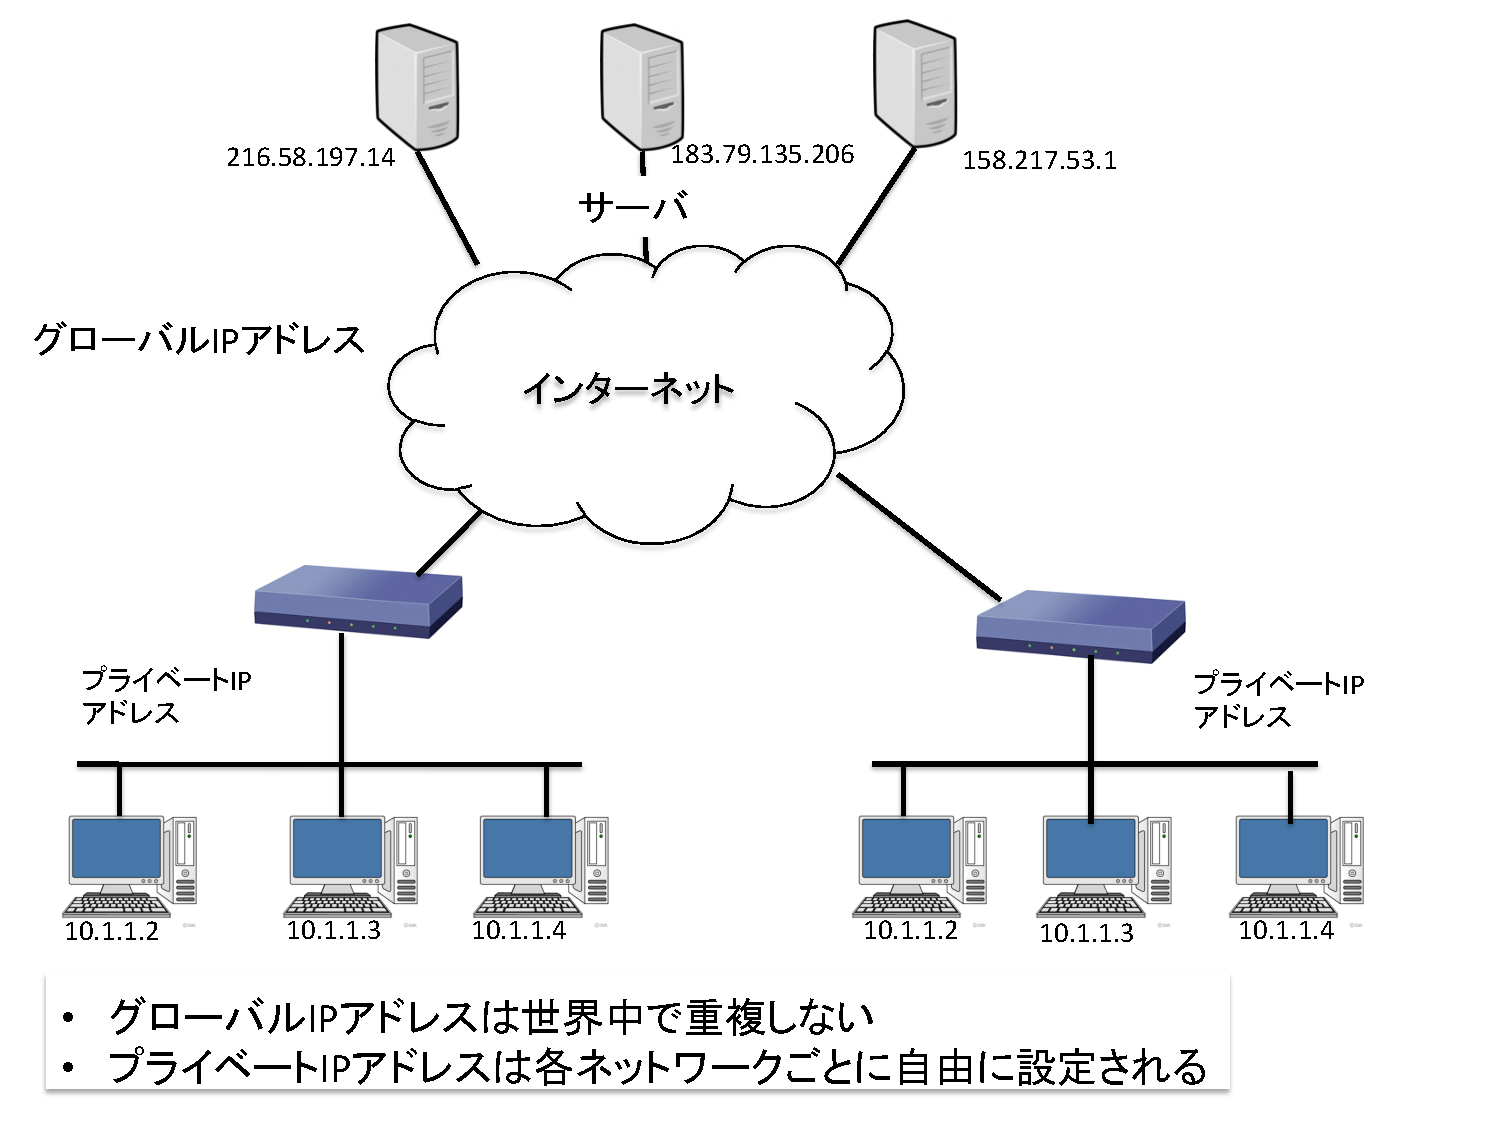
\includegraphics[width=14cm]{globalIP.pdf}
 \end{center}
 \caption{グローバルIPとプライベートIP}
 \label{glovalIP}
\end{figure}


\section{ルータ}
上の説明において,異なるネットワーク同士は直接通信できないと説明した.
しかし,異なるネットワークであるはずのグローバルIPアドレスに対してpingコマンドにより疎通を確認することができた.
また,私たちは日常においてインターネットを使用する際,無線LANなどから設定されたプライベートアドレスを用いて,インターネット上に存在するWebサイトなどのWebサービスを利用している.
これらのネットワークを越える通信はルータによって実現される.
ルータは異なるネットワーク間においてデータを中継する機器であり,インターネットに接続されるルータは外側にグローバルIPアドレス,内側にプライベートIPアドレスを割り当てられる.
このルータを用いることで,複数のネットワークで構成されるインターネット上においても,ルータが通信経路を中継することで目的の端末までデータを届けることができる(図\ref{router}).
こういった仕組みから,私たちはインターネット上の離れたネットワークに存在するサービスを利用することができる.
実際に通信経路を確認するため,例としてネットワーク経路を調べるtraceroute(tracert)コマンドを使用して関西大学のサーバまでの経路を確認する.

\begin{figure}[tbp]
 \begin{center}
  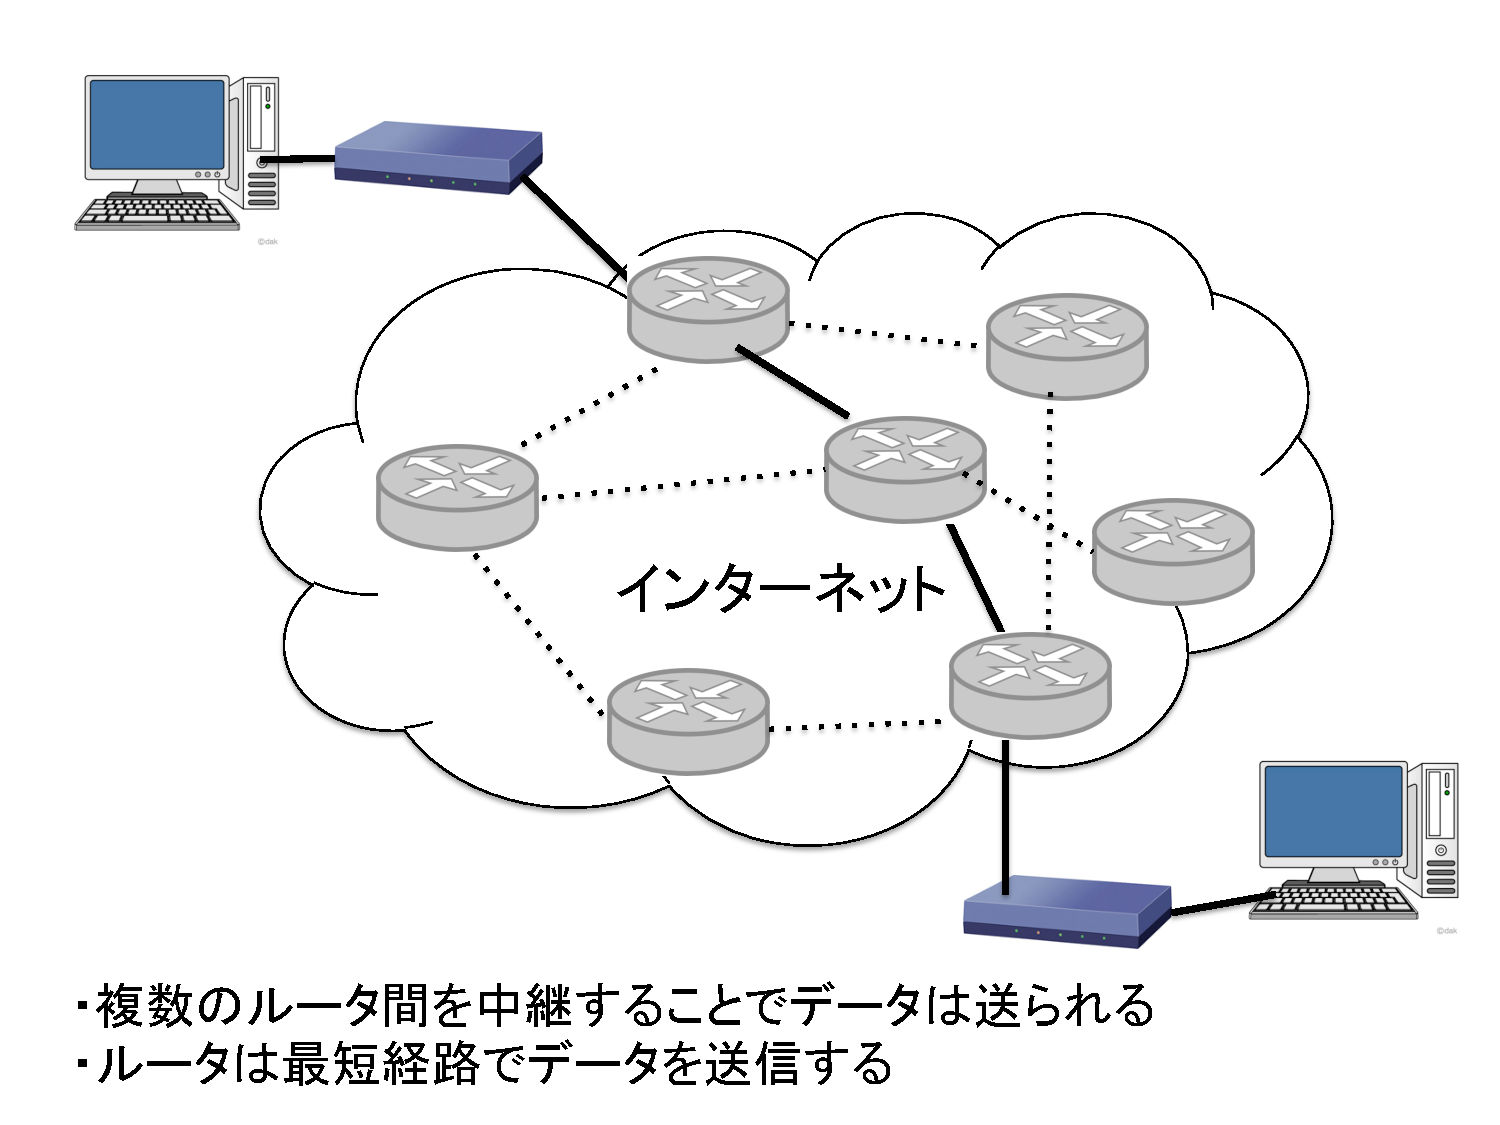
\includegraphics[width=10cm]{routing.pdf}
 \end{center}
 \caption{ルータによるデータの転送}
 \label{router}
\end{figure}
\newpage
Macは以下のコマンドを入力する.
\begin{screen}
\begin{verbatim}
# traceroute sh.edu.kutc.kansai-u.ac.jp
traceroute to sh.edu.kutc.kansai-u.ac.jp (158.217.53.13), 64 hops max, 52 
byte packets
 1  witccnt003.itc.kansai-u.ac.jp (172.29.70.203)  2.003 ms  0.975 ms  0.960 
 ms
 2  172.29.143.254 (172.29.143.254)  2.111 ms  2.154 ms  2.371 ms
 3  158.217.103.254 (158.217.103.254)  3.114 ms  3.504 ms  2.996 ms
 4  172.17.5.240 (172.17.5.240)  4.834 ms  4.463 ms  4.421 ms
 5  158.217.4.1 (158.217.4.1)  4.249 ms  3.509 ms  3.742 ms
 6  sh.edu.kutc.kansai-u.ac.jp (158.217.53.13)  2.920 ms !Z  2.992 ms !Z  
 4.961 ms
 \end{verbatim}
\end{screen}

windowsは以下のコマンドを入力する.
%結果を変更すること
\begin{screen}
\begin{Verbatim}[frame=single]
> traceroute sh.edu.kutc.kansai-u.ac.jp
sh.edu.kutc.kansai-u.ac.jp[158.217.53.13]へのルートをトレースしています
経由するホップ数は最大30です:
1  1ms 3ms   2ms  witccnt003.itc.kansai-u.ac.jp [172.29.70.203]
2  2ms  5ms  1ms  172.29.143.254
3  3ms  2ms  3ms  158.217.103.254
4  9ms  4ms  4ms  172.17.5.240
5  3ms  3ms  4ms  158.217.4.1
6  3ms  3ms  4ms  sh.edu.kutc.kansai-u.ac.jp [158.217.53.13]
トレースを完了しました。
\end{Verbatim}
\end{screen}
traceroute(tracert)コマンドの結果から,宛先までの経路が中継されていることが確認できる.

\section{ドメイン情報}
前の説明で宛先に関西大学のドメインを指定したように,インターネット上のサービスを利用する際はIPアドレスを指定するより,アドレスに対応付けられたドメイン名を使用することが一般的である.
また,このドメインについては,whoisサービスにより所有先の情報を調べることができる.
whoisサービスは,登録者情報,ネームサーバホスト情報,担当者情報などを確認することができる.
また,代表的なものとして,ANSI(\verb| http://whois.jprs.jp/ |)やJPRS(\verb|http://whois.ansi.co.jp/|)などがWebサービスを提供している.
(Unix系OSの場合,whoisコマンドを使用することでも検索することができる.)\par
ドメイン情報を調べるwhoisサービスの検索方法を説明する.
まず,インターネットブラウザからJPRSを検索し,検索結果からJPRS WHOIS /JPRSを選択する(図\ref{whois1}).
次に,ドメイン名登録情報検索に検索キーワードとして,関西大学のドメインであるkansai-u.ac.jpを入力し,検索ボタンを押下する(図\ref{whois2}).
検索結果からドメインの登録情報を確認することができる(図\ref{whois3}).

\begin{figure}[htbp]
 \begin{center}
  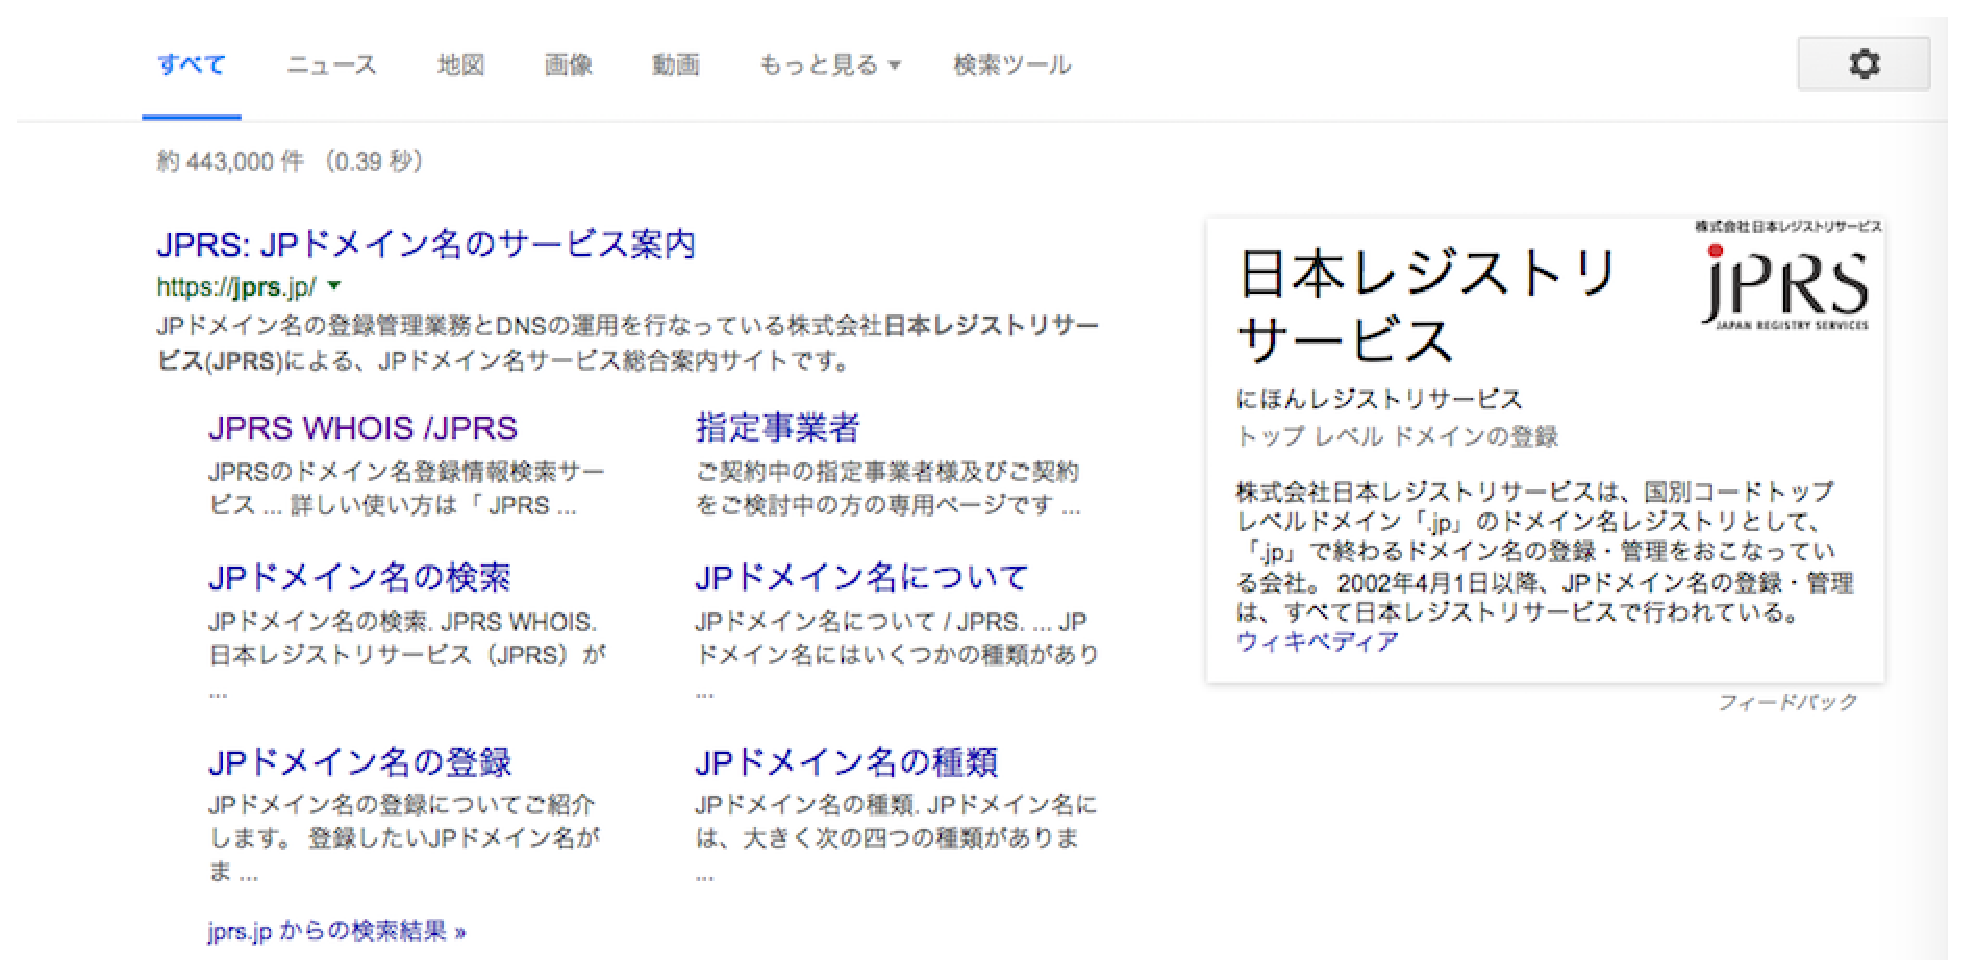
\includegraphics[width=15cm]{whois1.eps}
 \end{center}
 \caption{JPRSの検索}
 \label{whois1}
\end{figure}


\begin{figure}[htbp]
 \begin{center}
  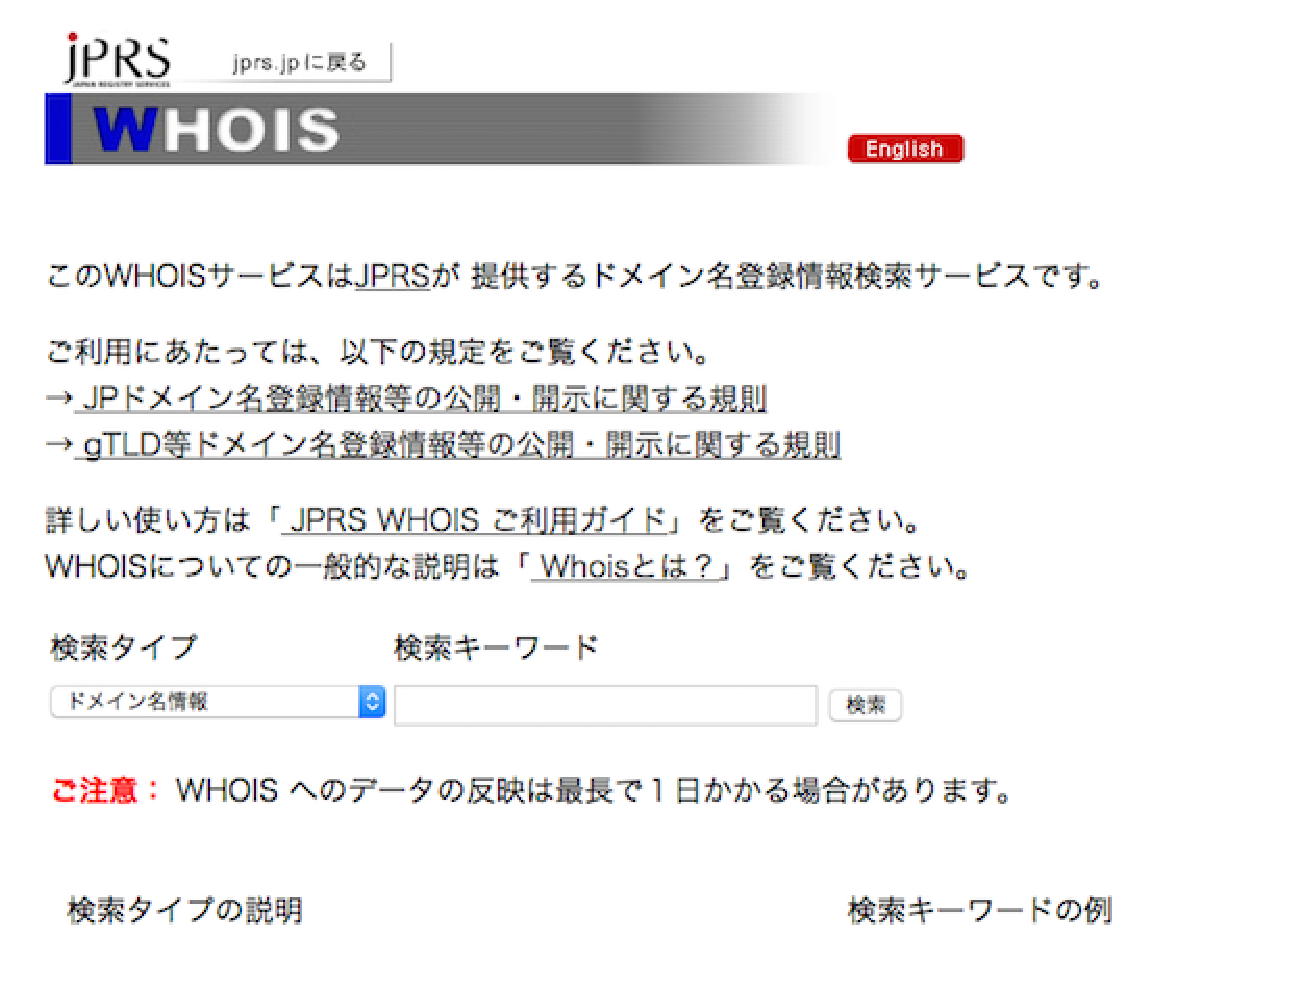
\includegraphics[width=12cm]{whois2.eps}
 \end{center}
 \caption{ドメイン名登録情報検索}
 \label{whois2}
\end{figure}

\begin{figure}[htbp]
 \begin{center}
  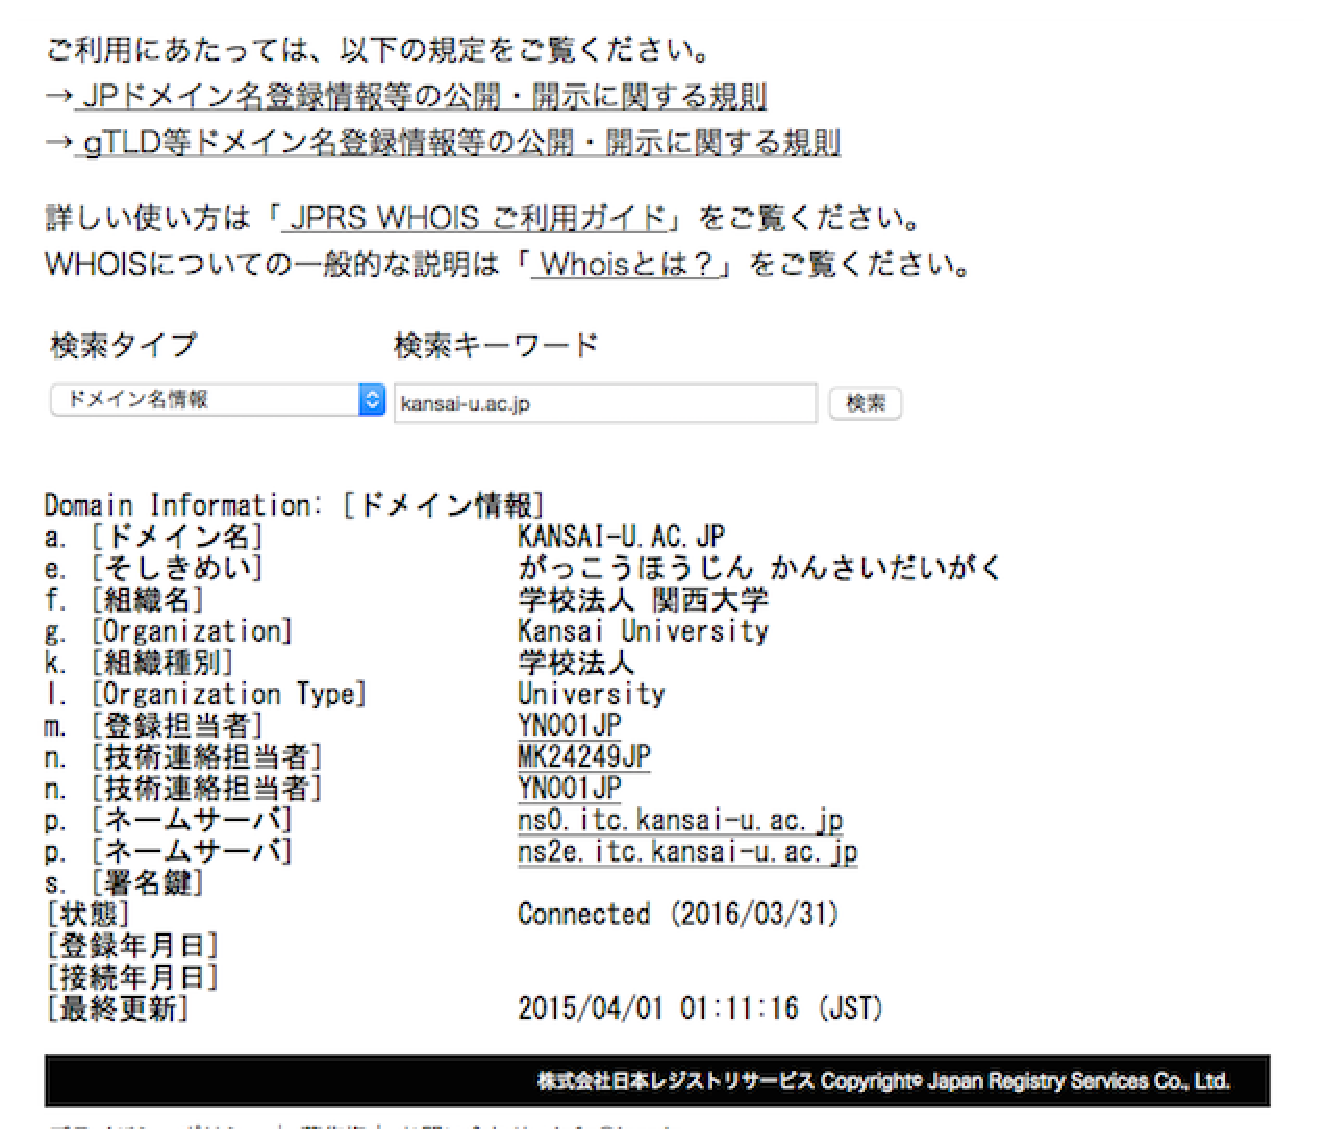
\includegraphics[width=13cm]{whois3.eps}
 \end{center}
 \caption{ドメイン情報結果}
 \label{whois3}
\end{figure}

\newpage

\section{NATとNAPT}
%グローバルとプライベートで通信を行う仕組み
ここでは,ルータの機能としてグローバルIPアドレスとプライベートIPアドレスの通信について説明する.\par
前述のIPアドレス枯渇問題から,プライベートIPアドレスの割り当てを説明したが,
グローバルIPアドレスが振られるインターネット側からは,プライベートIPアドレスを認識することはできない.
そこで,グローバルネットワークとプライベートネットワークの通信を可能にするため,ルータのNAT(Network Address Translation)機能を用いている.
インターネットに繋がるルータには,外側にグローバルIPアドレス,内側にプライベートIPアドレスを割り当てられているが,
NATはこのグローバルIPアドレスとプライベートIPアドレスの変換を行う.\par
NATの仕組みとして,プライベートIPアドレスが割り振られた端末が,インターネット上のグローバルIPアドレスと通信を行う場合について説明する.\par
まず,プライベートIPアドレスから送信があった場合,ルータは送信元となるプライベートIPアドレスはルータの外側にあるグローバルIPアドレスに変換する.そして,送信元がグローバルIPアドレスとなったデータは,インターネット上の宛先へと送信される.
次に,インターネット上から送信元に対して返信があった場合は,変換された送信元であるルータの外側のアドレスに対して返信される.そして,返信を受け取ったルータは送信先を本来の送信元であるプライベートIPアドレスに転送することで,インターネット上との通信を可能にする.\par
このように,ルータが中継となってアドレスを変換することで,プライベートIPアドレスとグローバルIPアドレス間で通信を行うことを可能にする(図\ref{nat}).

しかし,NATでのアドレス変換は一つのグローバルIPアドレスに対して,一つのプライベートIPアドレスを対応づけるため,
グローバル側との通信は一つの端末のみに限られてしまう.
そこで,NAT機能の拡張としてNAPT(Network Address Port Translation)の機能が用いられる.
NAPTは,一つの端末しか接続できない問題に対応するため,ポート番号を用いる.
ポート番号はサーバが提供するサービスを識別する番号である.
このポート番号を端末ごとに割り当て,番号をもとに宛先の端末を識別することで,ポート番号を利用して複数の端末により通信を行うことが可能となる.
\begin{figure}[htbp]
 \begin{center}
 %\vspace{-1cm}
  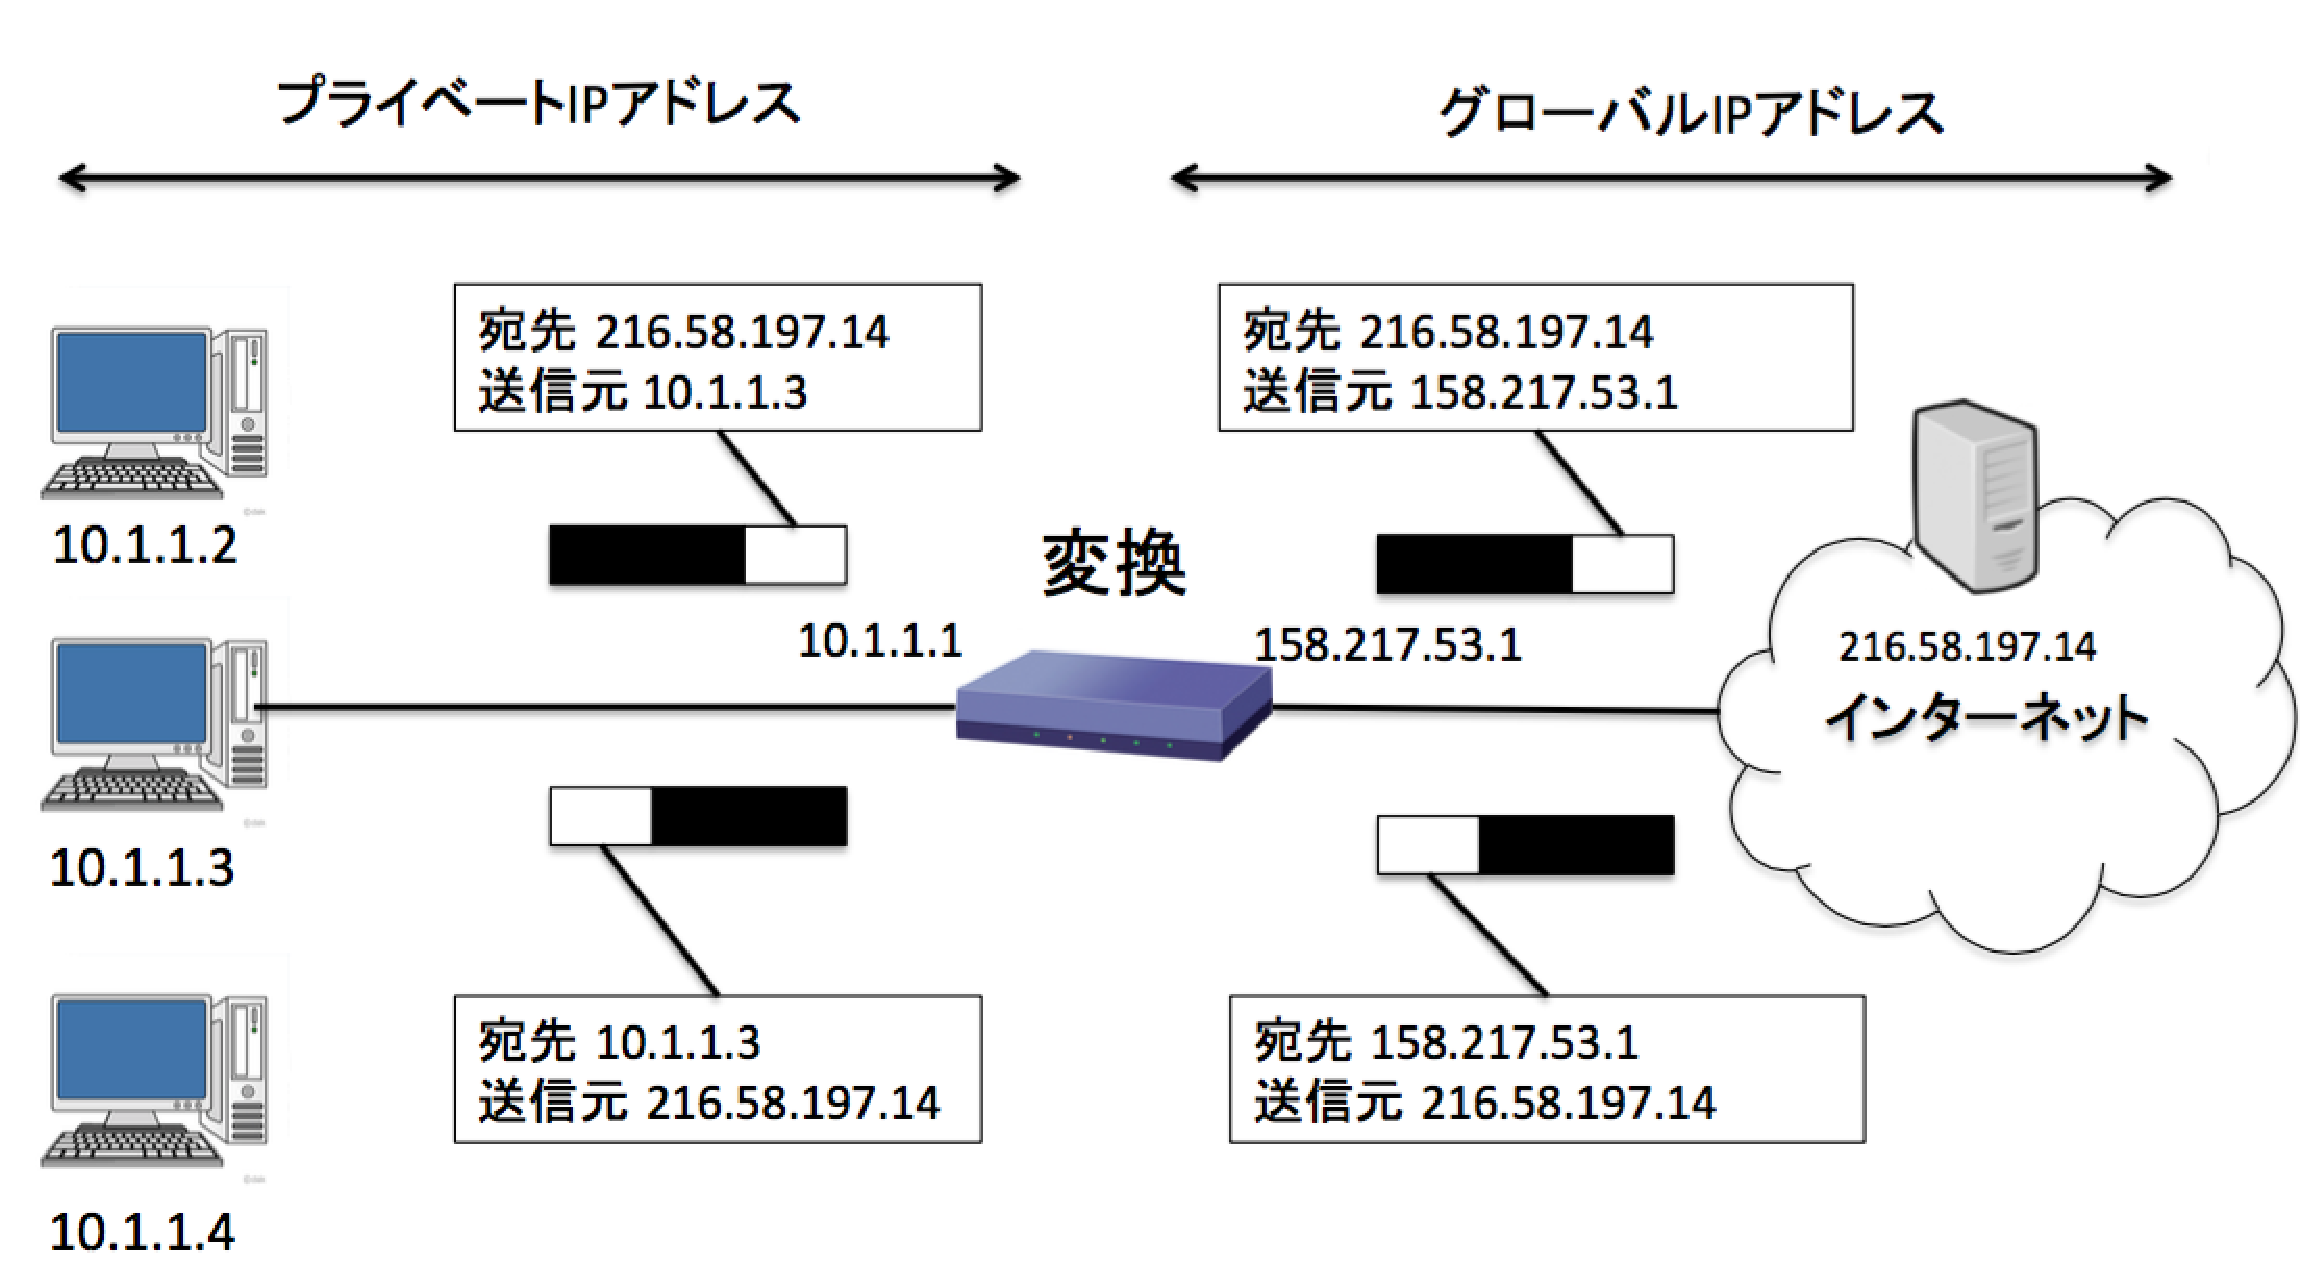
\includegraphics[width=14cm]{nat.eps}
 \end{center}
 \caption{NATによるアドレス変換}
 \label{nat}
\end{figure}

\subsection{DHCP}
ここまで,プライベートIPアドレスを利用した技術の説明をした.
プライベートIPアドレスの使用に伴い,ネットワークで管理される端末数も増加し,IPアドレスの管理も大変になる.
しかし,日常生活で利用する際にIPアドレスを設定する機会はほとんどない.
多くの場合,実際のIPアドレスの設定はDHCP(Dynamic Host Configuration Protocol)により行われる.
また,設定機能を持った機器をDHCPサーバと呼ぶ.
これは,IPアドレスやDNSなどのネットワーク情報を持っており,ネットワークに接続した端末に対して設定情報を提供する.
また,端末がネットワークから離脱するとDHCPリソースを更新する.
このようにDHCPは,IPアドレスの割り当てなど,ネットワーク情報を自動的に管理することができる.

%VPNについて
\section{VPN(Virtual Private Network)}
自宅など,外部のネットワークからゼミ内のプライベートIPアドレスが割り振られているマシンなどを操作する場合はネットワークが異なるため,直接的に利用することはできない.
そこでVPNという技術を用いることで,異なるネットワーク同士を仮想的に同一のネットワークに属しているように見せかけ,
異なるネットワークの端末と通信することができるようになる.\par
VPNによる通信の仕組みとして,トンネリングによりネットワークを繋いでいる.
トンネリングでは,もとの通信内容にヘッダが加えられ,加えられたヘッダにより通信内容はカプセル化される.このカプセル化を用いることで接続元でカプセル化を行い,接続先でカプセル化を解除し通信内容を取り出すことで,ネットワーク同士をトンネルで繋いだように見立てて使用することが可能となる.
さらに,データをカプセル化する際は,データを暗号化することで安全にネットワークを越えて通信することが可能となる(図\ref{vpn}).
VPNで利用されるプロトコルには,IPsec/PPTP/L2TP/L2F/MPLSなどがある.
\begin{figure}[htbp]
 \begin{center}
  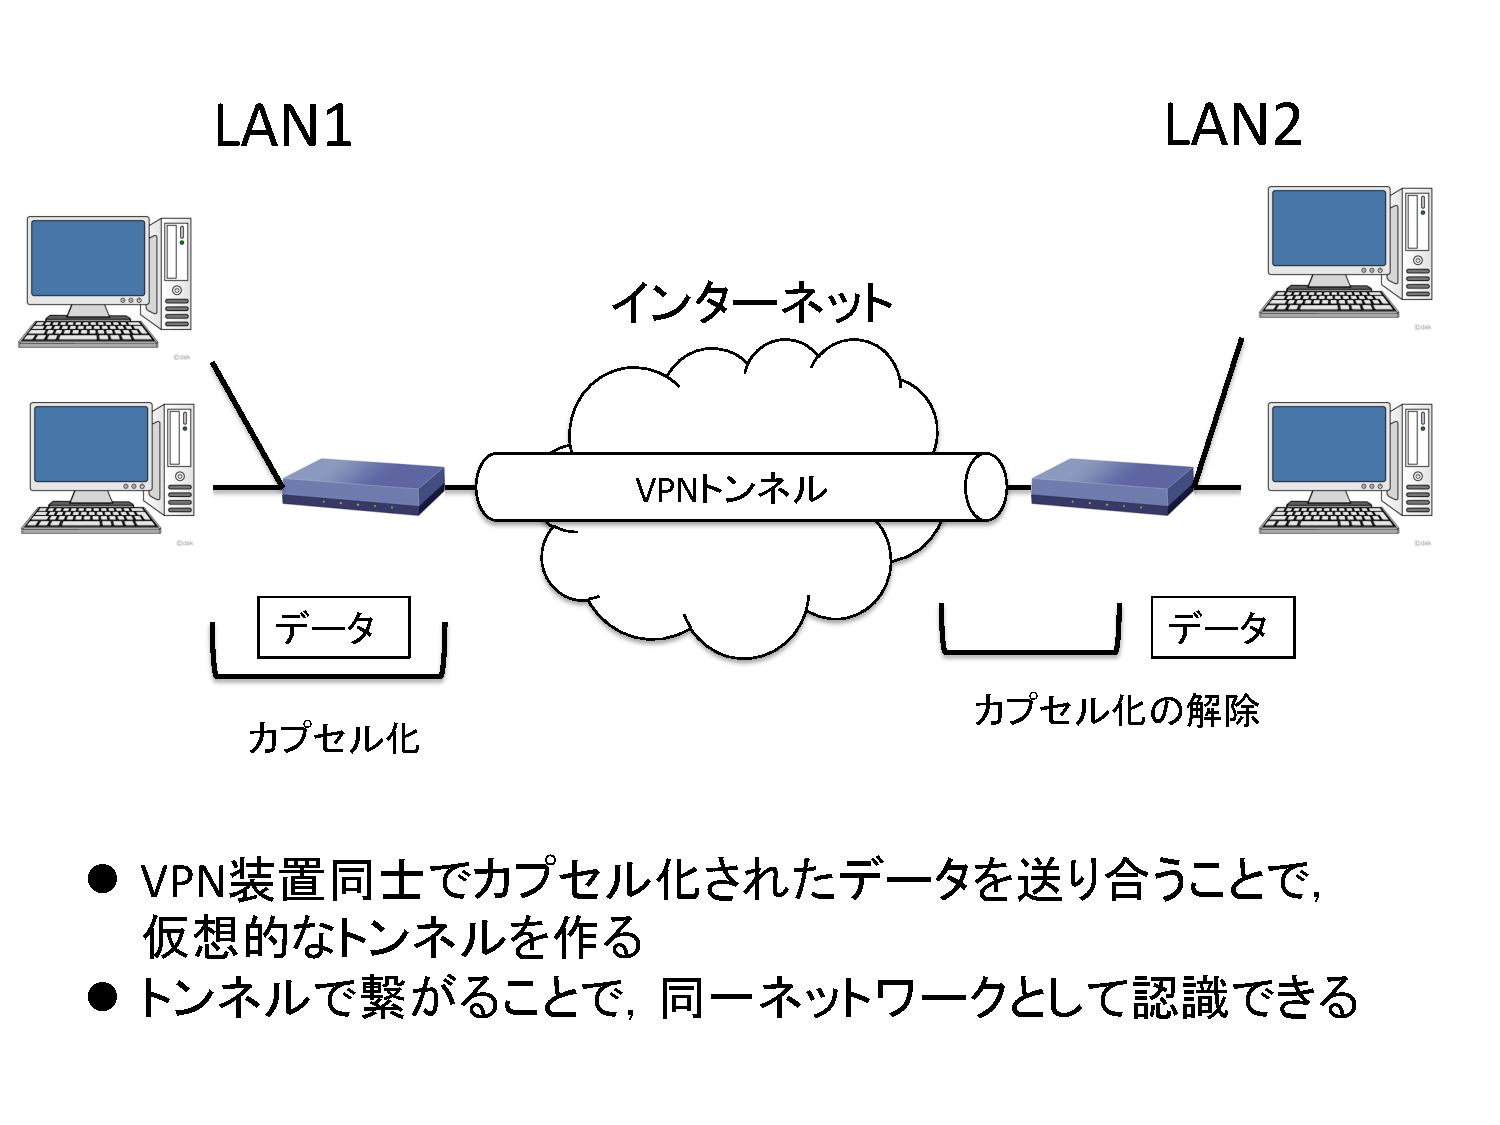
\includegraphics[width=13cm]{vpn.pdf}
 \end{center}
 \caption{VPNの概要}
 \label{vpn}
\end{figure}

\newpage

\subsection{小林ゼミのVPN}
小林ゼミのVPN環境において利用可能なプロトコルはL2TP Over IPSecとPPTPがある.
Macはいずれのプロトコルも利用することが可能である.ただし,L2TP Over IPSecはPPTP
よりもセキュアなため前者の使用を推奨する.はじめに,VPNの設定に必要な情報を表\ref{servers}に示す.
サーバアドレスはcririn.firefly.kutc.kansai-u.ac.jpと同じ158.217.77.225を使用する.
アカウント名とパスワードはXoopsにログインする時と同じものを使用する.共有シークレットは口頭で伝える.
\begin{table}[htbp]
\begin{center}
\caption{VPN設定に必要な情報}
\label{servers}
\begin{tabular}{| l | l |c|}
	\hline
	項目 & 値  \\ \hline
	サーバアドレス & 158.217.77.225 \\ 
	 アカウント名 & Xoopsで使用するアカウント名 \\
  	パスワード & Xoopsで使用するパスワード \\ 
	 共有シークレット & ****** \\ \hline
\end{tabular}
\end{center}
\end{table}
\subsection{VPNの設定(Macの場合)}
システム環境設定からネットワークを開く(図\ref{Mvpn1}).次に+から新しいサービスを作成する.
新たに表示されたウィンドウでインタフェースをVPN,VPNタイプをL2TP Over IPSecかPPTPを選択,
サービス名は任意に入力して,作成を押す(図\ref{Mvpn2}).
新しいサービスが作成されたので,そのサービスを選択した状態で設定を入力する.構成はデフォルト,サーバアドレスは158.217.77.225,
アカウント名を入力する.次に認証設定を押す.
ここでL2TP over IPSecによるVPN構成の場合は,ユーザ認証でパスワード,コンピュータ認証で共有シークレットを入力する(図\ref{Mvpn4}).
PPTPによるVPN構成の場合はパスワードを入力する.
さらにPPTPの暗号化は自動(128ビットまたは40ビット)にする.
以上全ての項目を入力して,適応と接続を行う.またメニューバーにVPNの状況を表示をチェックすることで接続状態や接続時間が表示される.
これはVPN接続のショートカット機能も有しているのでチェックすることを推奨する(図\ref{Mvpn3}).
\begin{figure}[htbp]
 \begin{center}
  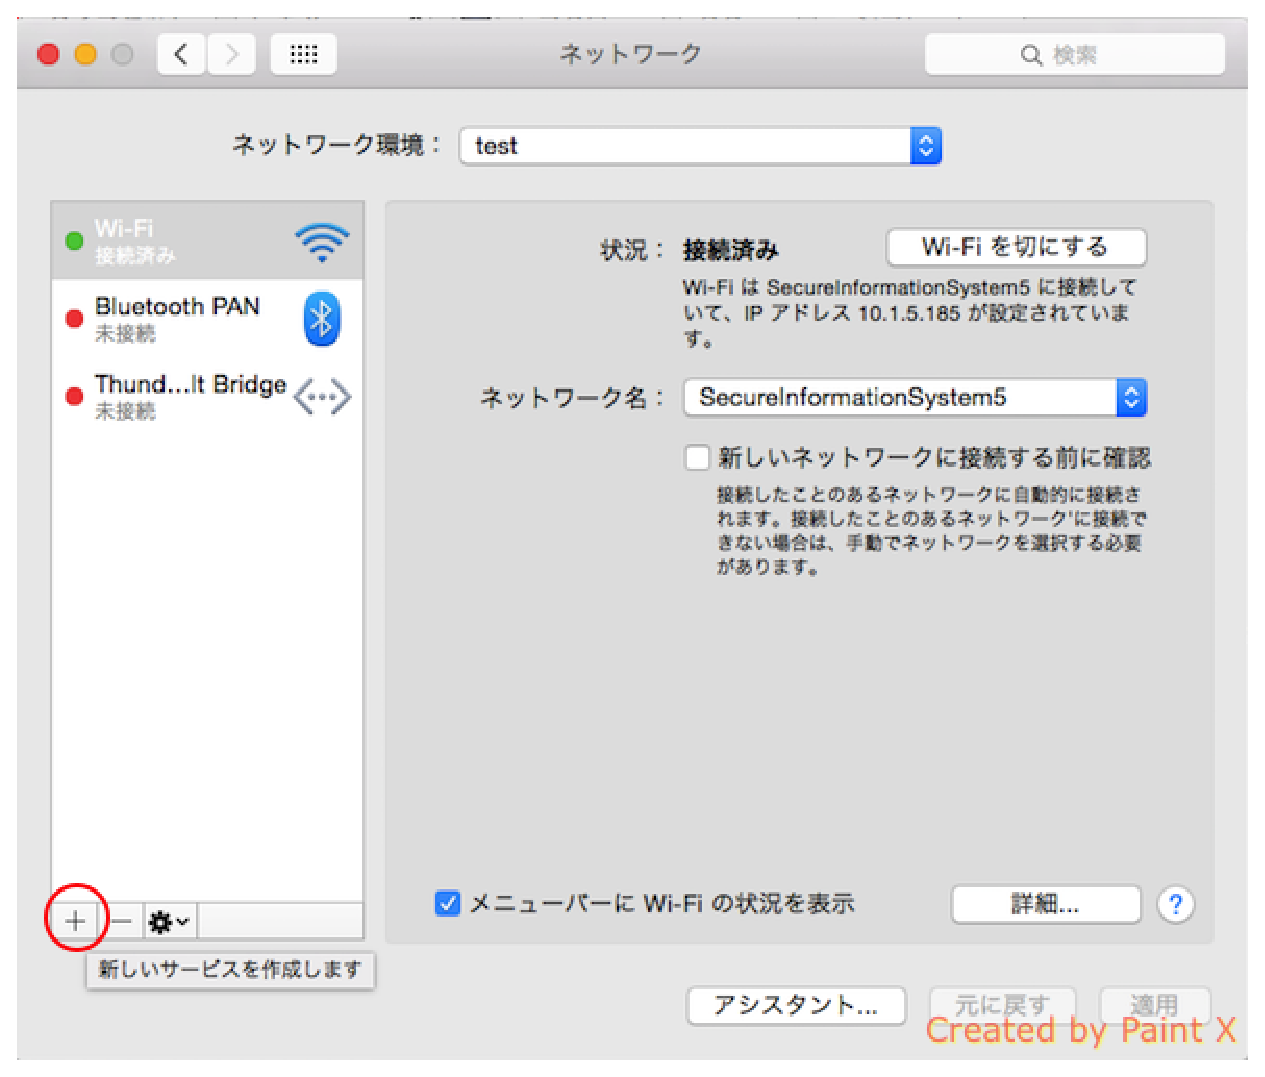
\includegraphics[width=13cm]{vpn1-mac.eps}
 \end{center}
 \caption{ネットワーク設定}
 \label{Mvpn1}
\end{figure}

\begin{figure}[htbp]
 \begin{center}
  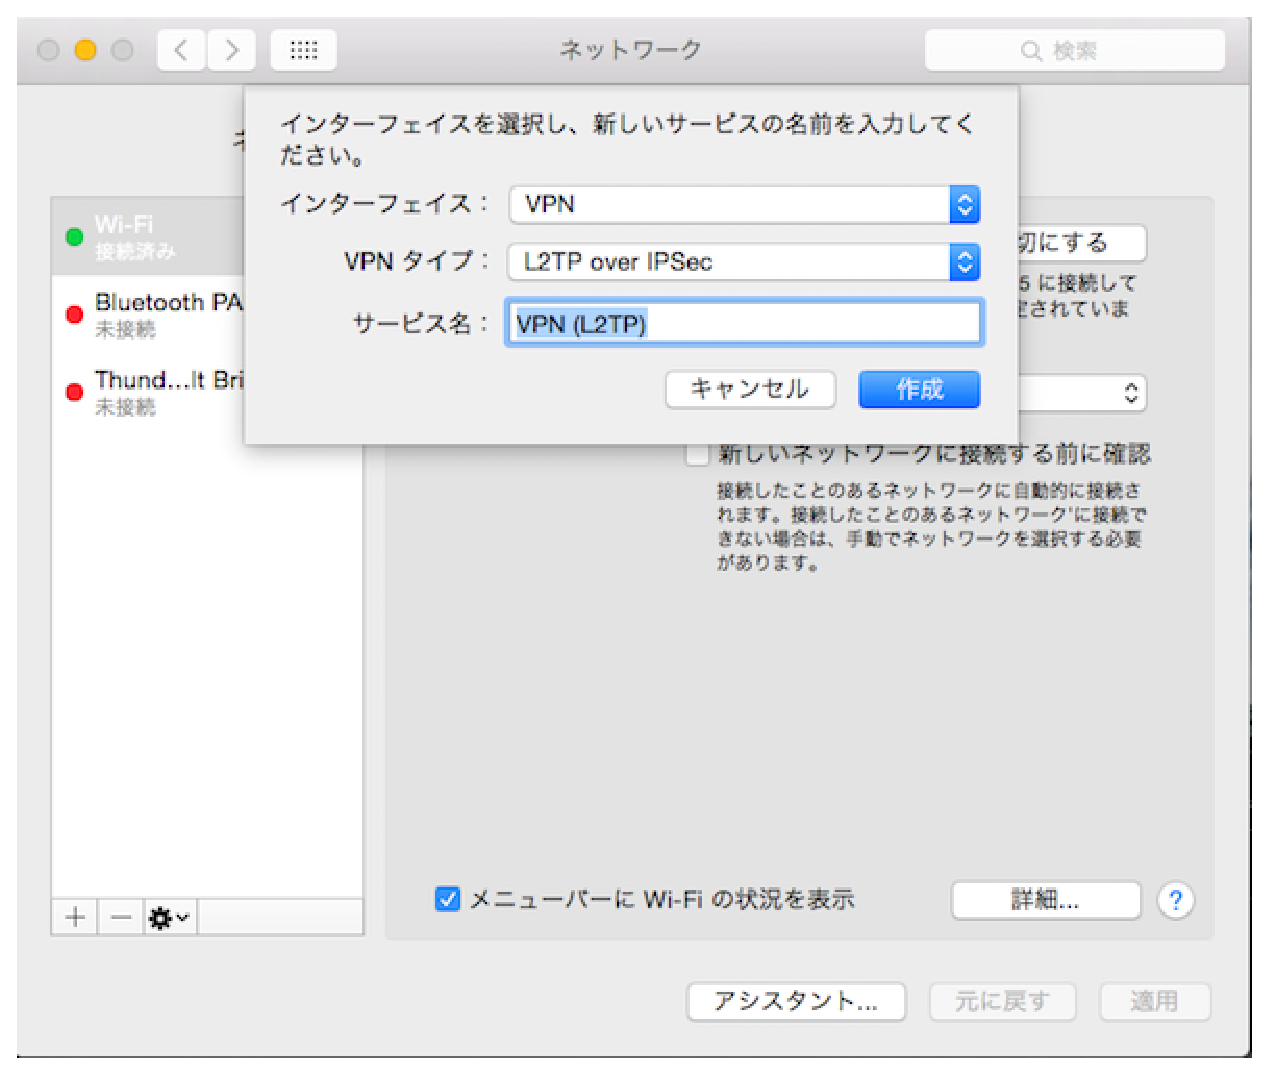
\includegraphics[width=13cm]{vpn2-mac.eps}
 \end{center}
 \caption{vpnサービスの作成}
 \label{Mvpn2}
\end{figure}

\begin{figure}[htbp]
 \begin{center}
  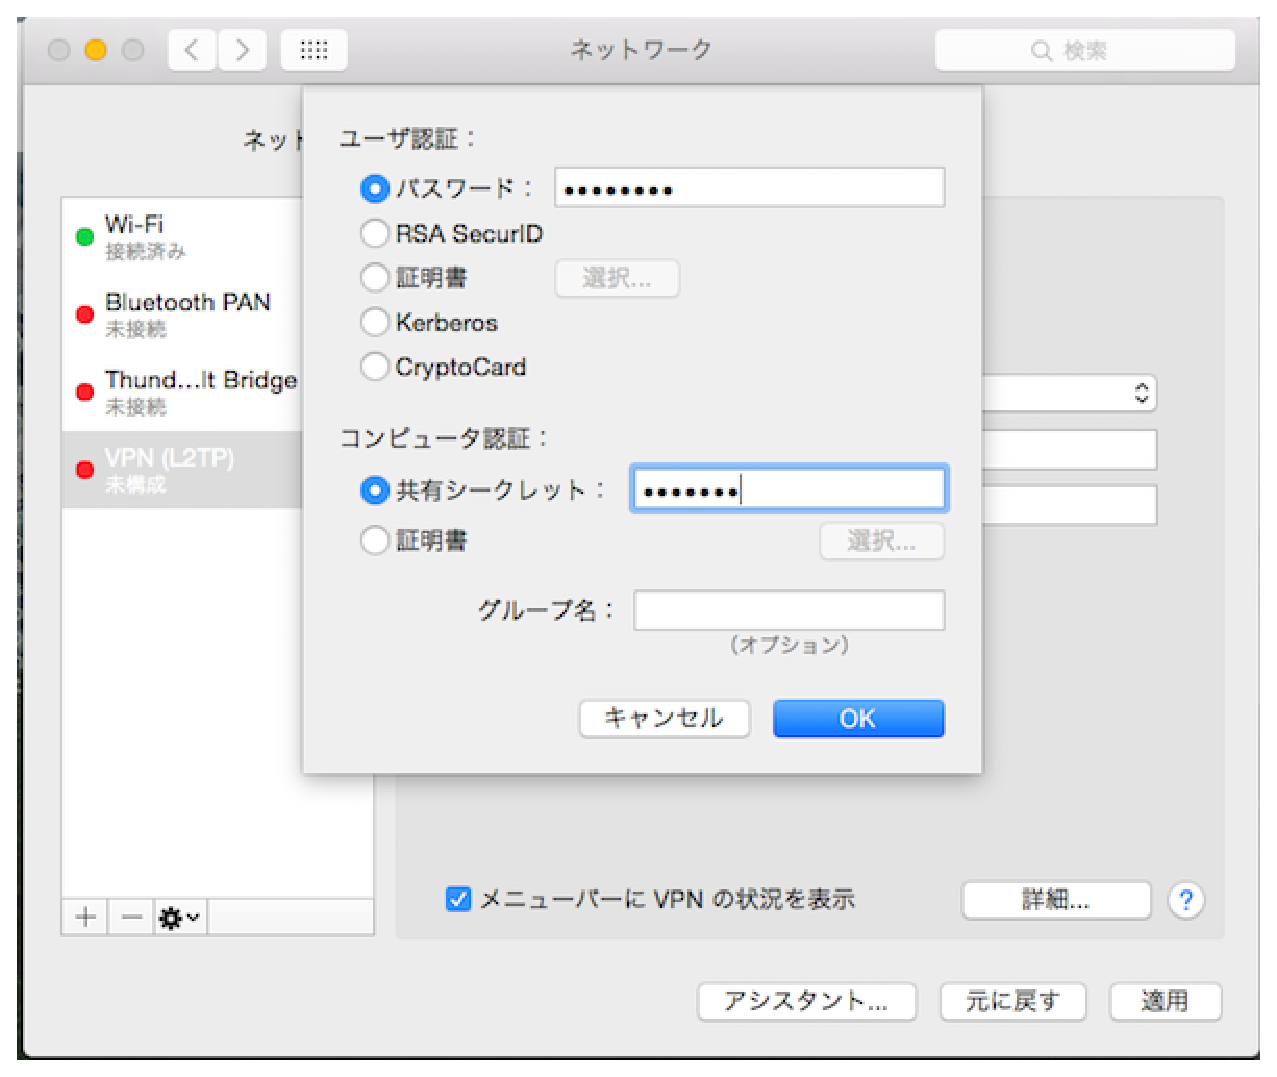
\includegraphics[width=13cm]{vpn4-mac.eps}
 \end{center}
 \caption{ L2TP Over IPSecの認証設定}
 \label{Mvpn4}
\end{figure}

\begin{figure}[htbp]
 \begin{center}
  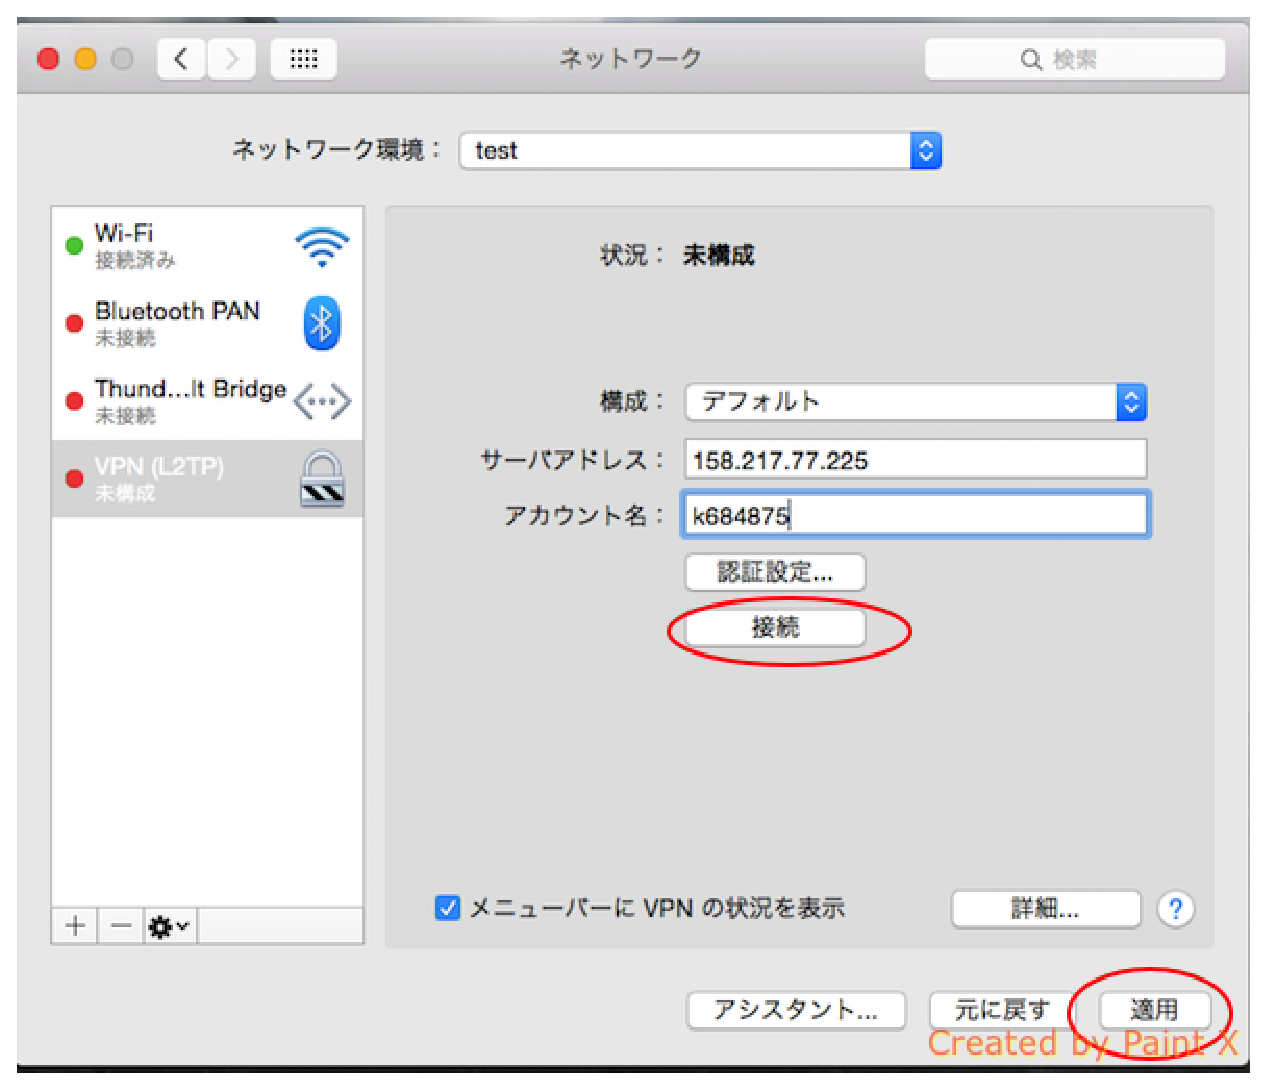
\includegraphics[width=13cm]{vpn3-mac.eps}
 \end{center}
 \caption{VPNの適応と接続}
 \label{Mvpn3}
\end{figure}

\newpage
\subsection{VPNの設定(Windows10の場合)}
ホーム画面左下のWindowsアイコンから設定をクリックする(図\ref{winvpn1}).
開いたウィンドウからネットワークとインターネットを選択する(図\ref{winvpn2}).
次に,開いたメニュー左のVPNからVPN接続を追加するを選択する(図\ref{winvpn3}).
VPNの設定ウィンドウについては,各項目に正しく入力する.それぞれ,VPNプロバイダーはwindows(ビルトイン).
接続名はVPN.サーバ名またはアドレスには158.217.77.225.VPNの種類はPPTP.ユーザ名とパスワードを入力し保存を押す(図\ref{winvpn4}).
ウィンドウを閉じると,関連設定のメニューにあるアダプターのオプションを変更を選択する(図\ref{winvpn5}).
作成したVPN設定のアイコンが表示されるのを確認し,アイコンの上で右クリックからプロパティを選択(図\ref{winvpn6}).セキュリティタブをクリックし,VPNの種類がPPTPになっているのを確認とデータの暗号化には暗号化が必要を選んでOKを押す(図\ref{winvpn7}).
最後に,ネットワークとインターネットのウィンドウから接続を選択し,接続中になっていることが確認できれば完了となる(図\ref{winvpn8}).

\begin{figure}[htbp]
 \begin{center}
  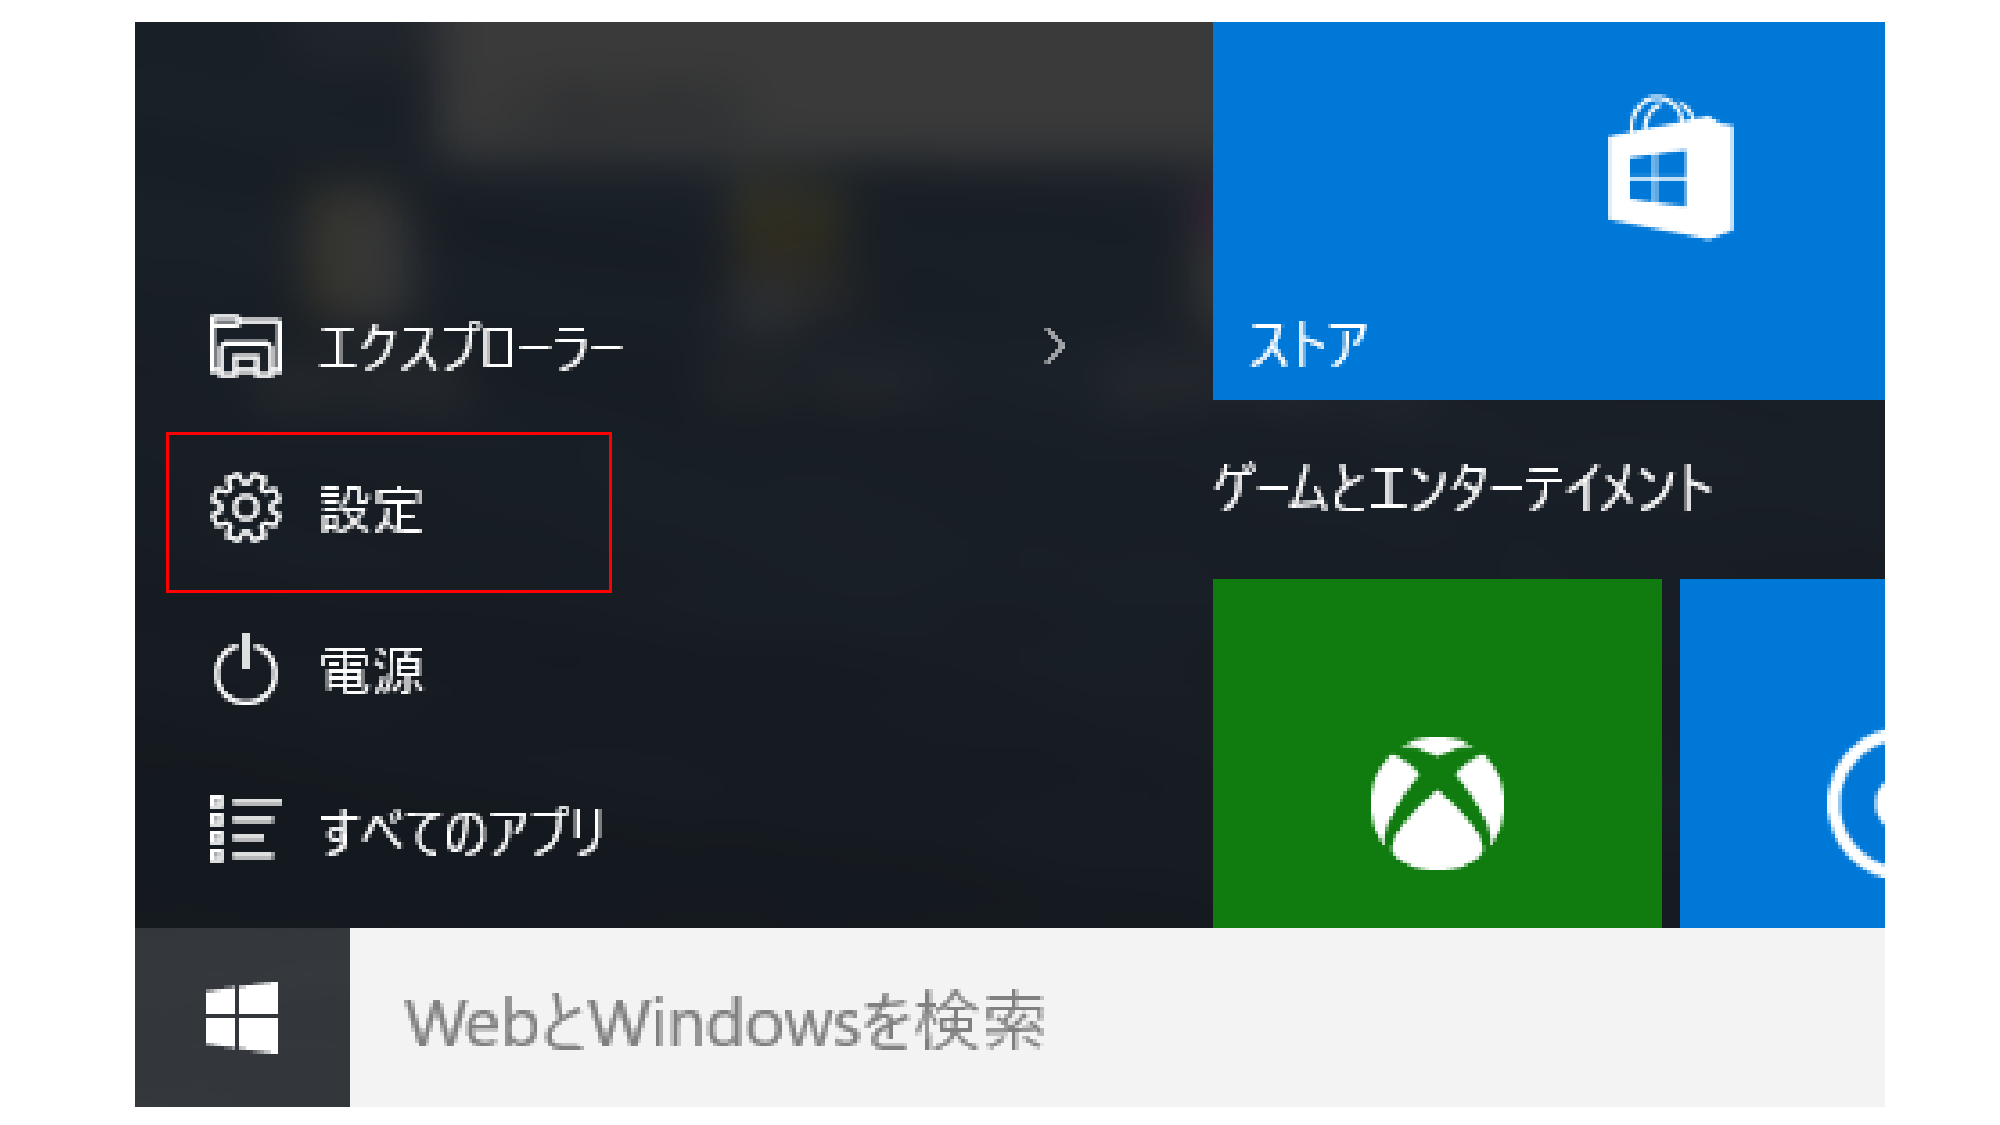
\includegraphics[width=12cm]{win-vpn1.pdf}
 \end{center}
 \caption{VPNの設定1}
 \label{winvpn1}
\end{figure}

\begin{figure}[htbp]
 \begin{center}
  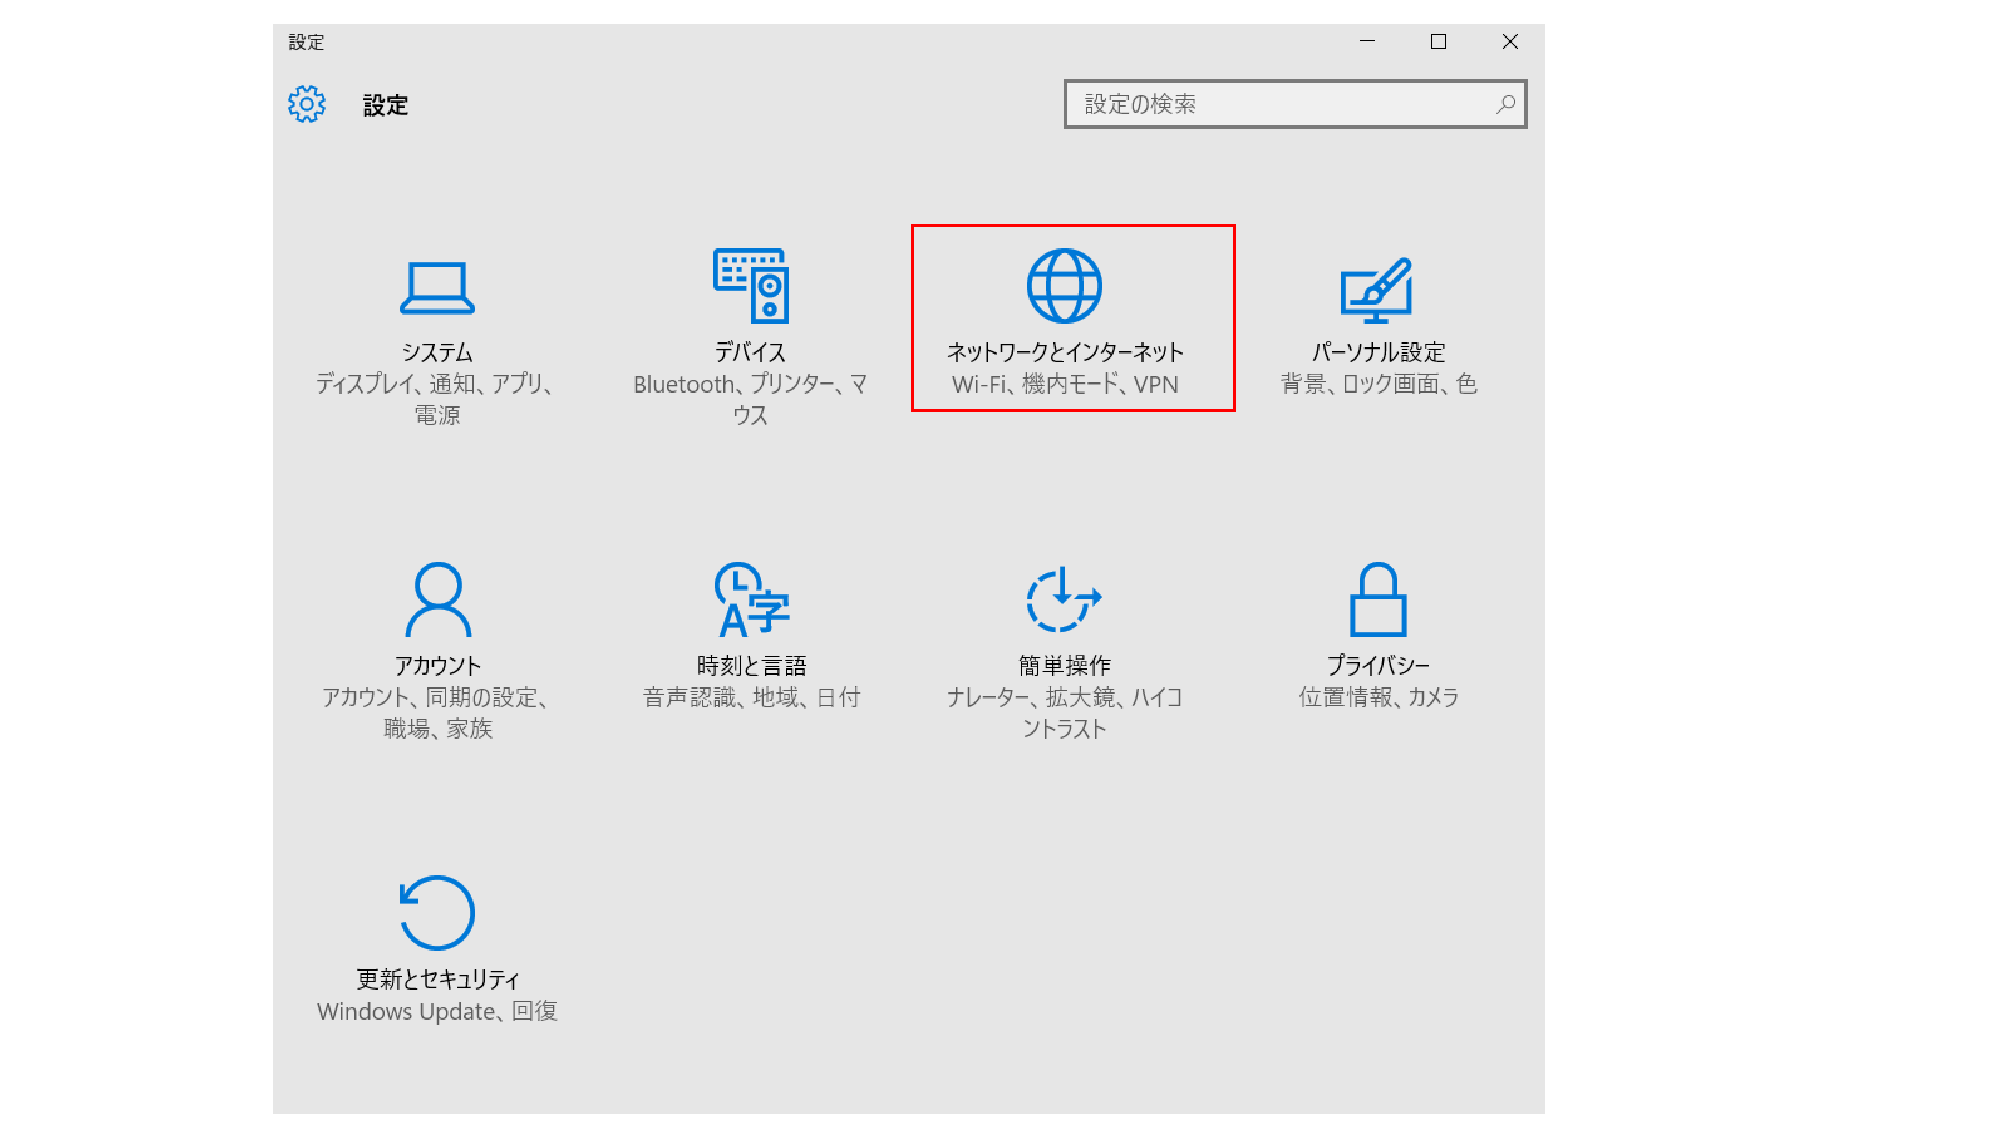
\includegraphics[width=15cm]{win-vpn2.pdf}
 \end{center}
 \caption{VPNの設定2}
 \label{winvpn2}
\end{figure}

\begin{figure}[htbp]
 \begin{center}
  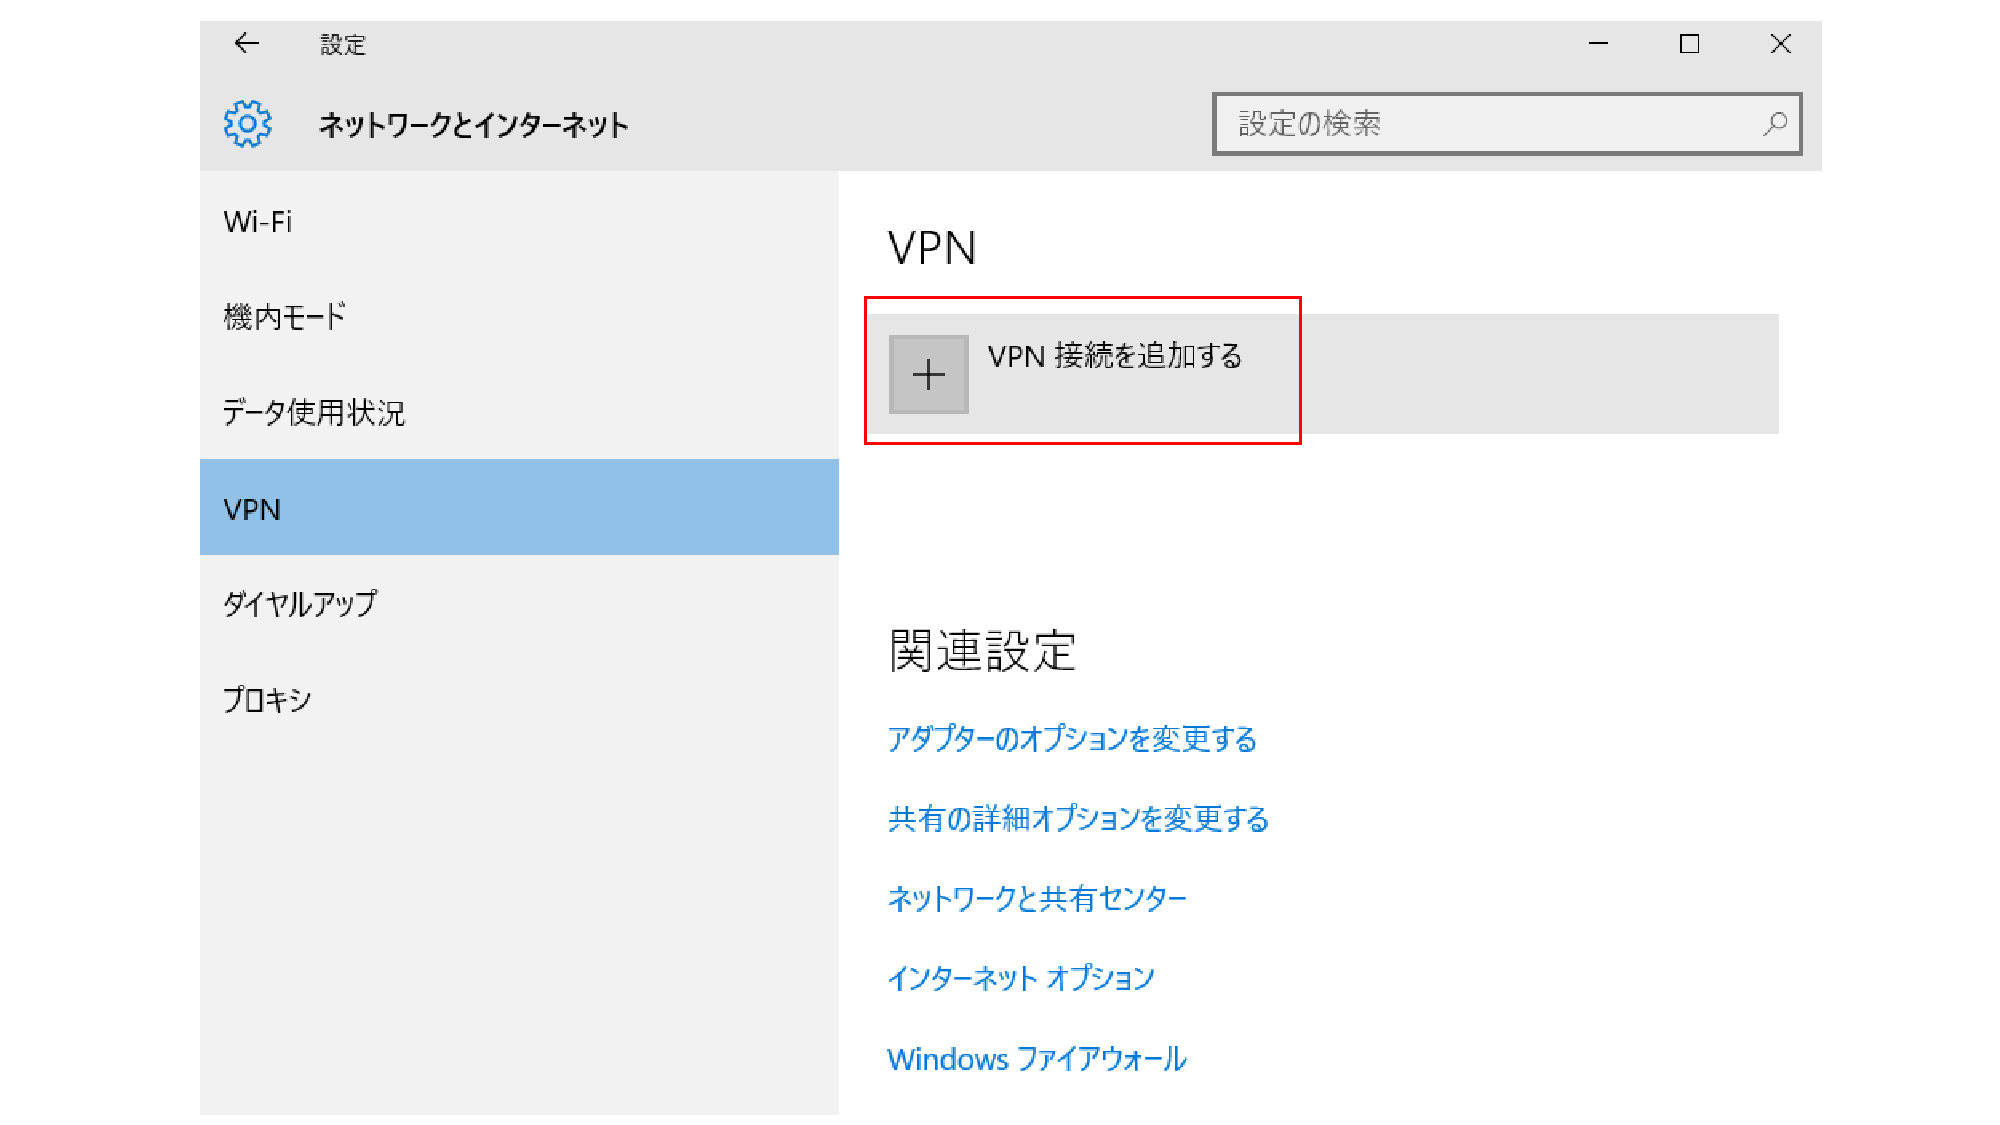
\includegraphics[width=17cm]{win-vpn3.pdf}
 \end{center}
 \caption{VPNの設定3}
 \label{winvpn3}
\end{figure}

\begin{figure}[htbp]
 \begin{center}
  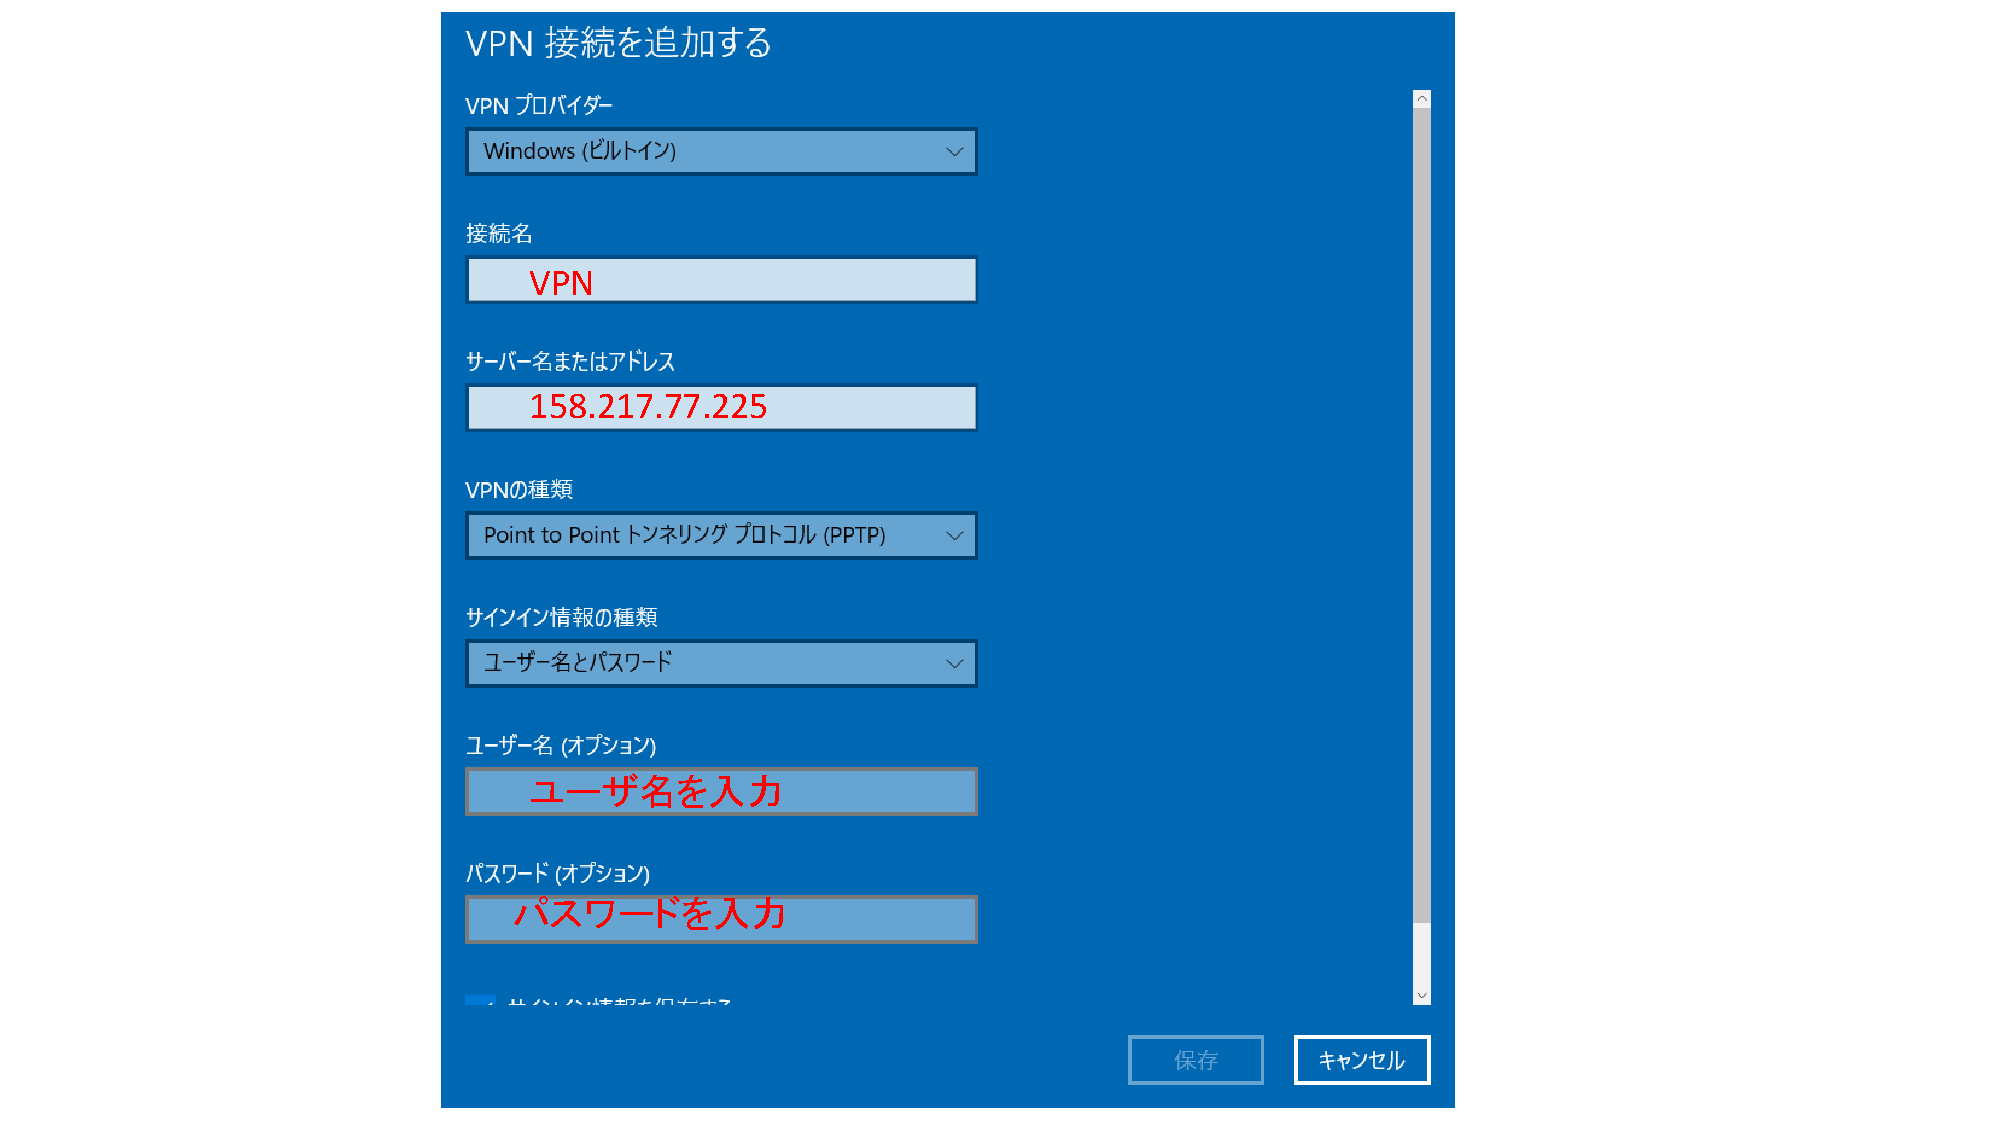
\includegraphics[width=18cm]{win-vpn4.pdf}
 \end{center}
 \caption{VPNの設定4}
 \label{winvpn4}
\end{figure}

\begin{figure}[htbp]
 \begin{center}
  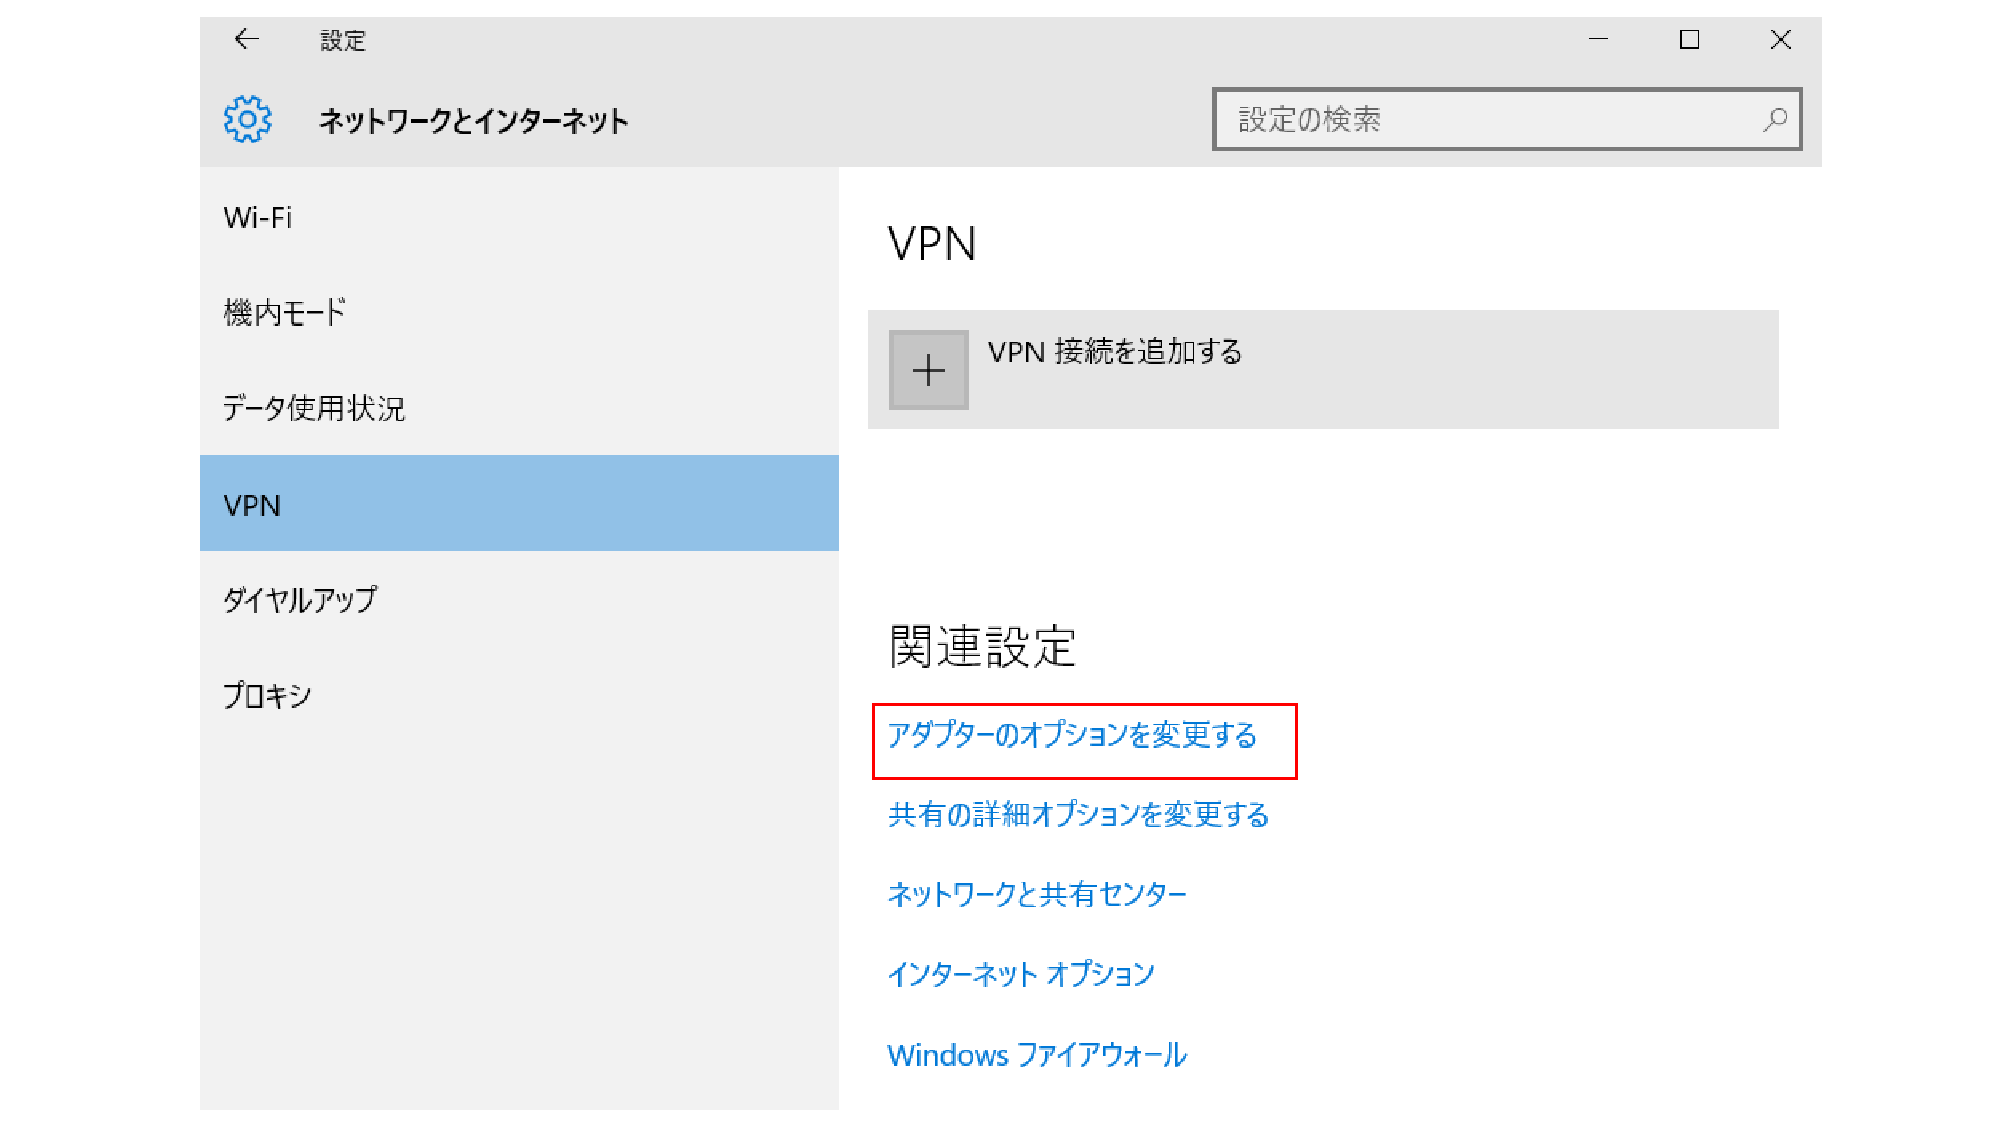
\includegraphics[width=15cm]{win-vpn5.pdf}
 \end{center}
 \caption{VPNの設定5}
 \label{winvpn5}
\end{figure}

\begin{figure}[htbp]
 \begin{center}
  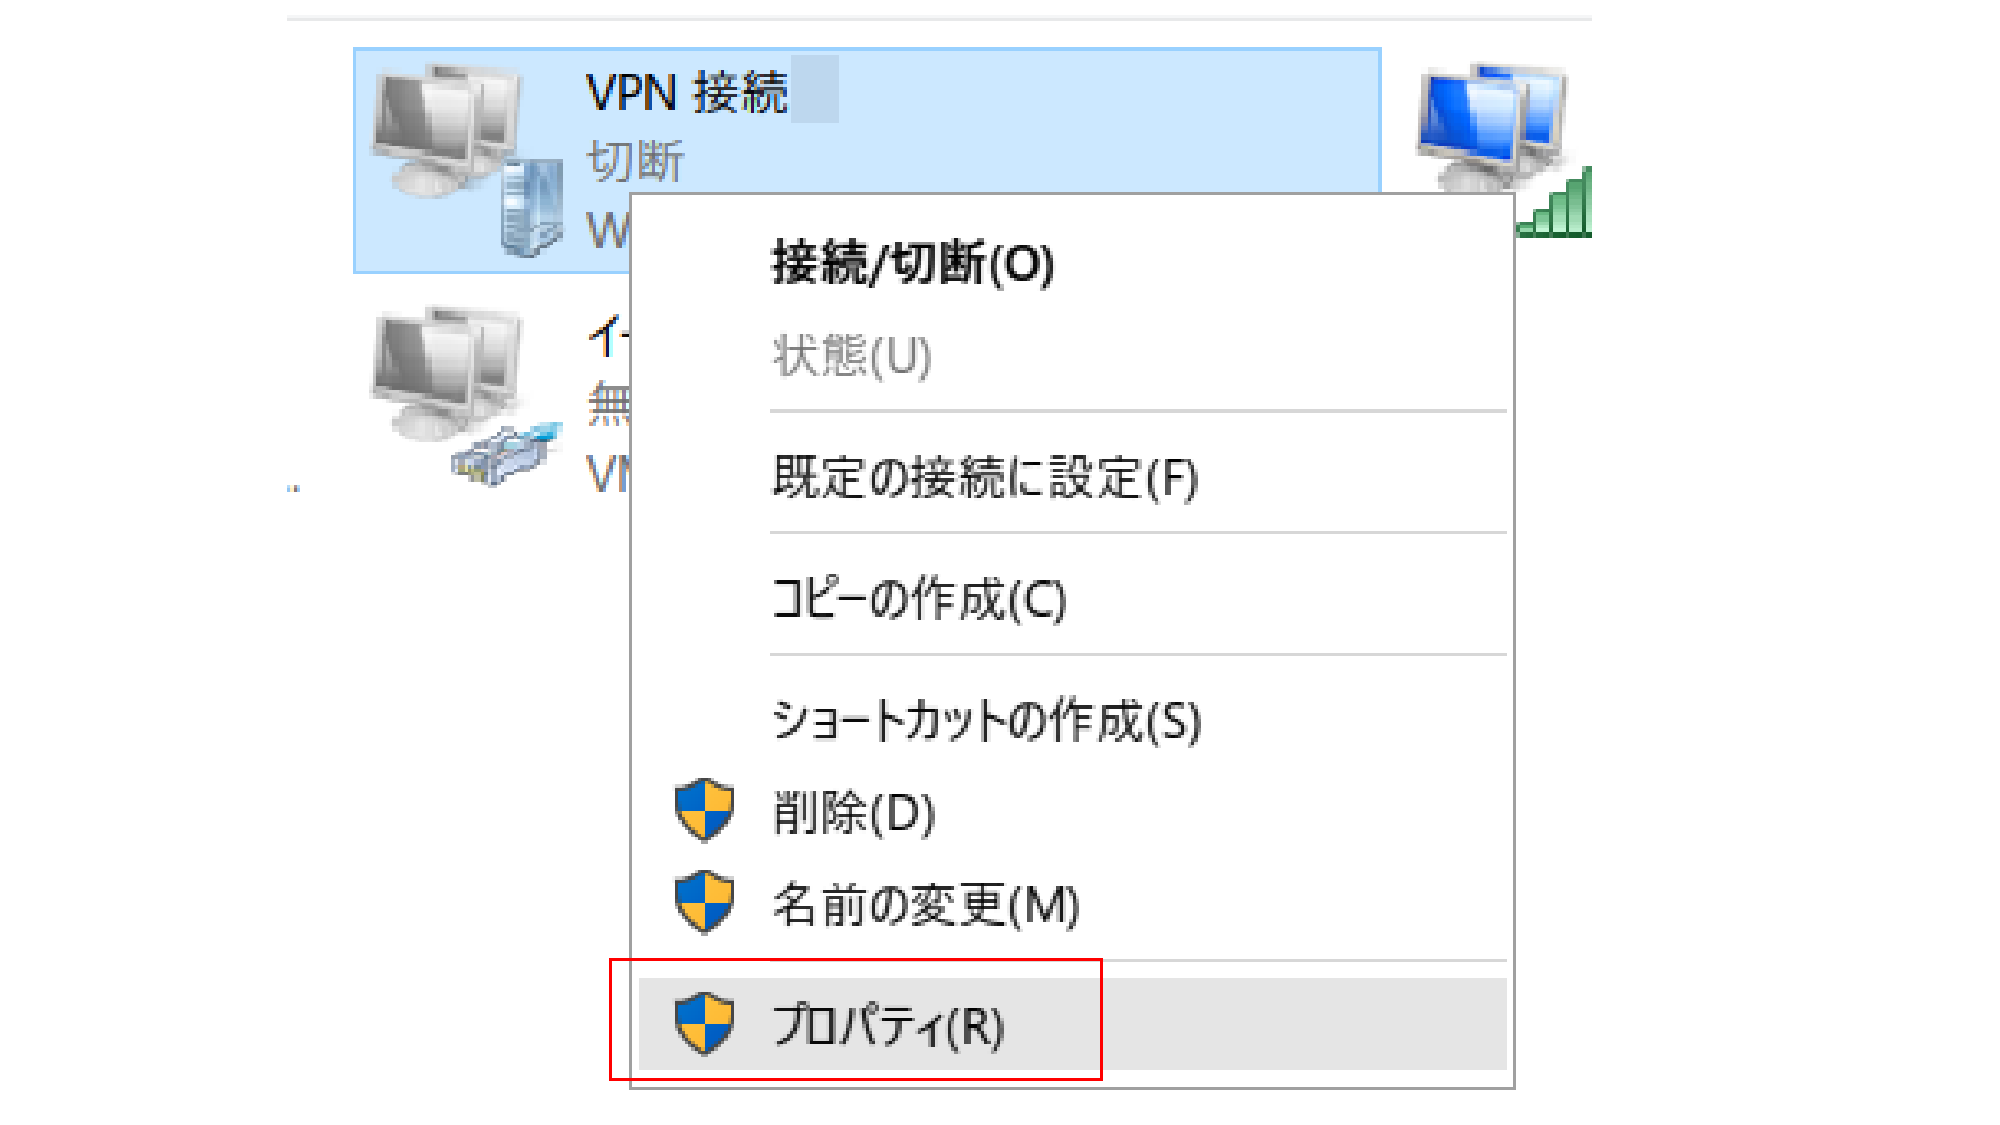
\includegraphics[width=17cm]{win-vpn6.pdf}
 \end{center}
 \caption{VPNの設定6}
 \label{winvpn6}
\end{figure}

\begin{figure}[htbp]
 \begin{center}
  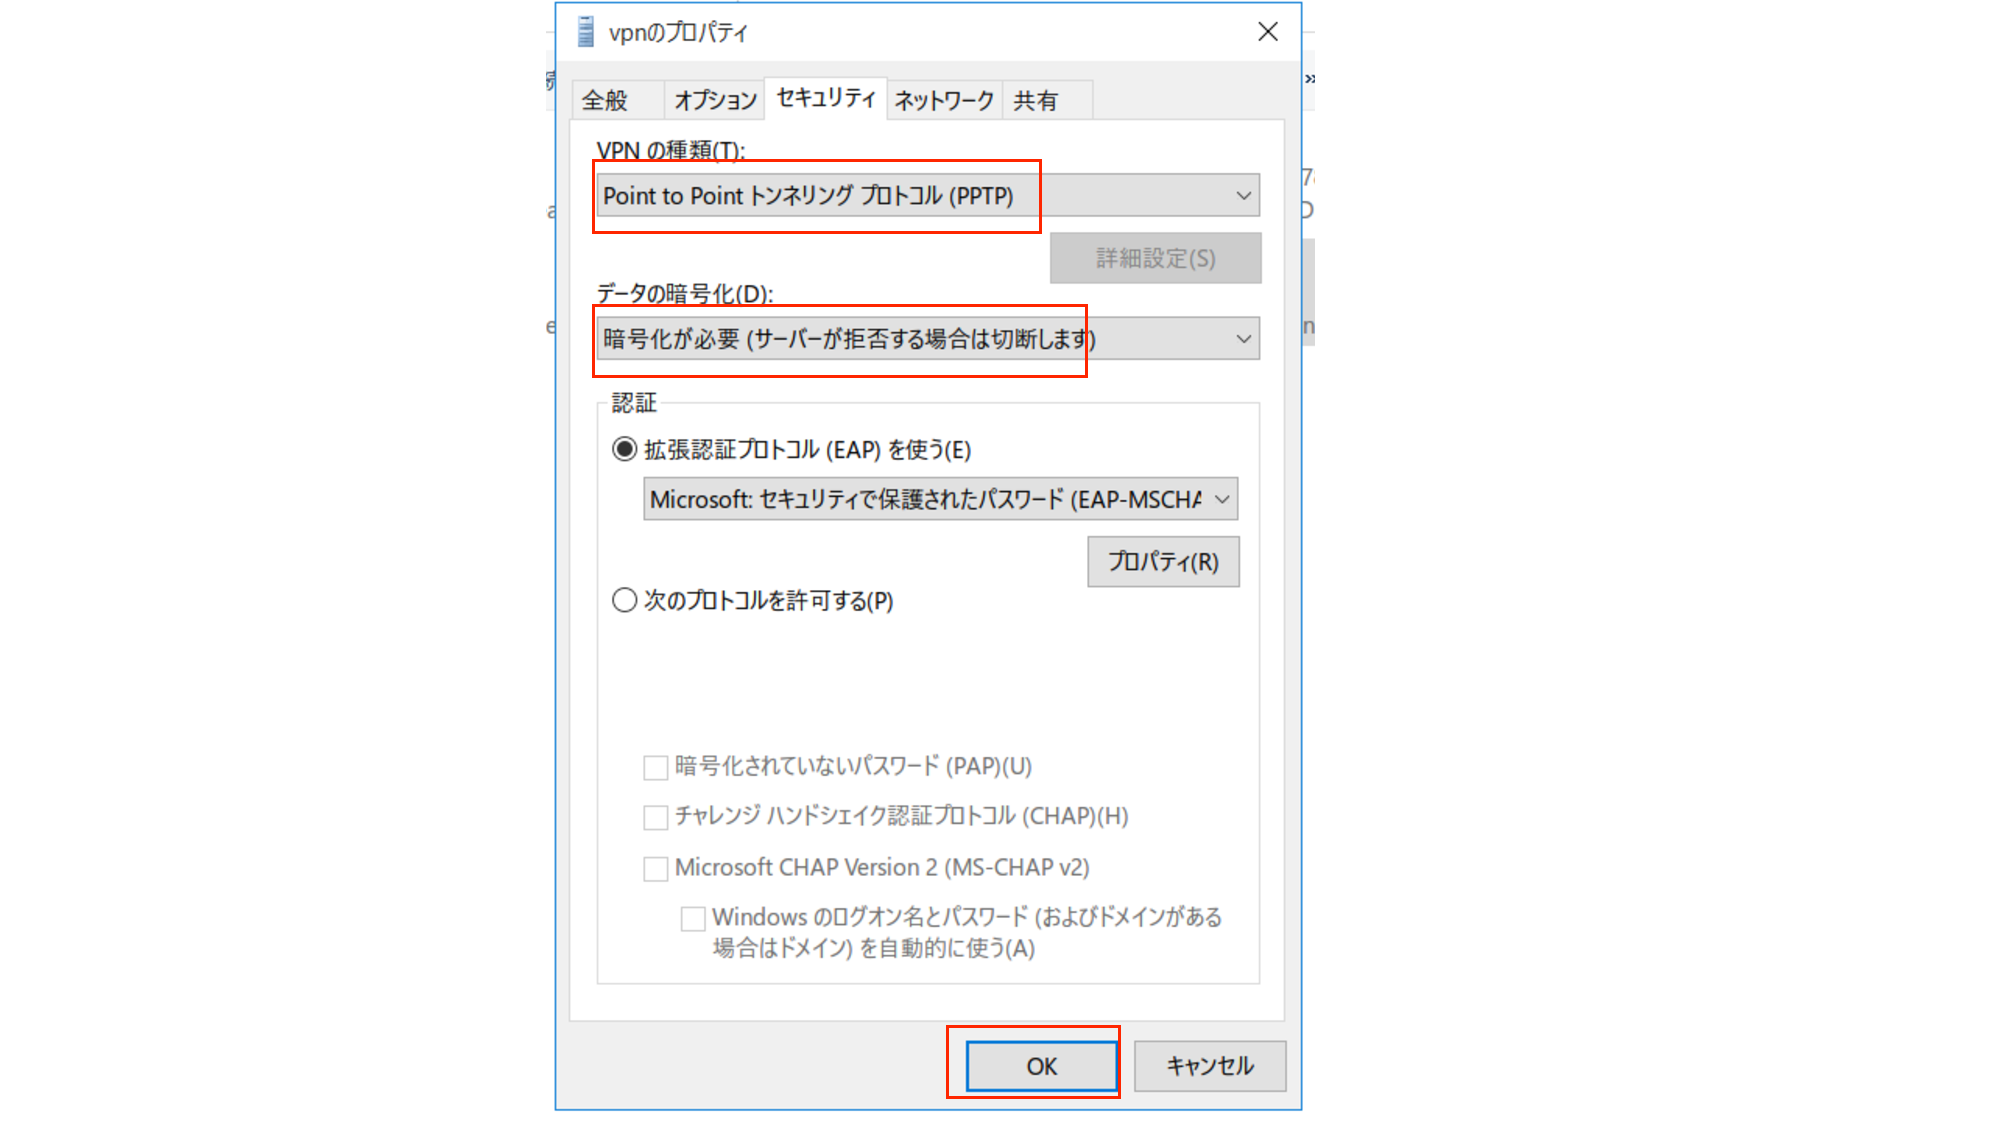
\includegraphics[width=19cm]{win-vpn7.pdf}
 \end{center}
 \caption{VPNの設定7}
 \label{winvpn7}
\end{figure}

\begin{figure}[htbp]
 \begin{center}
  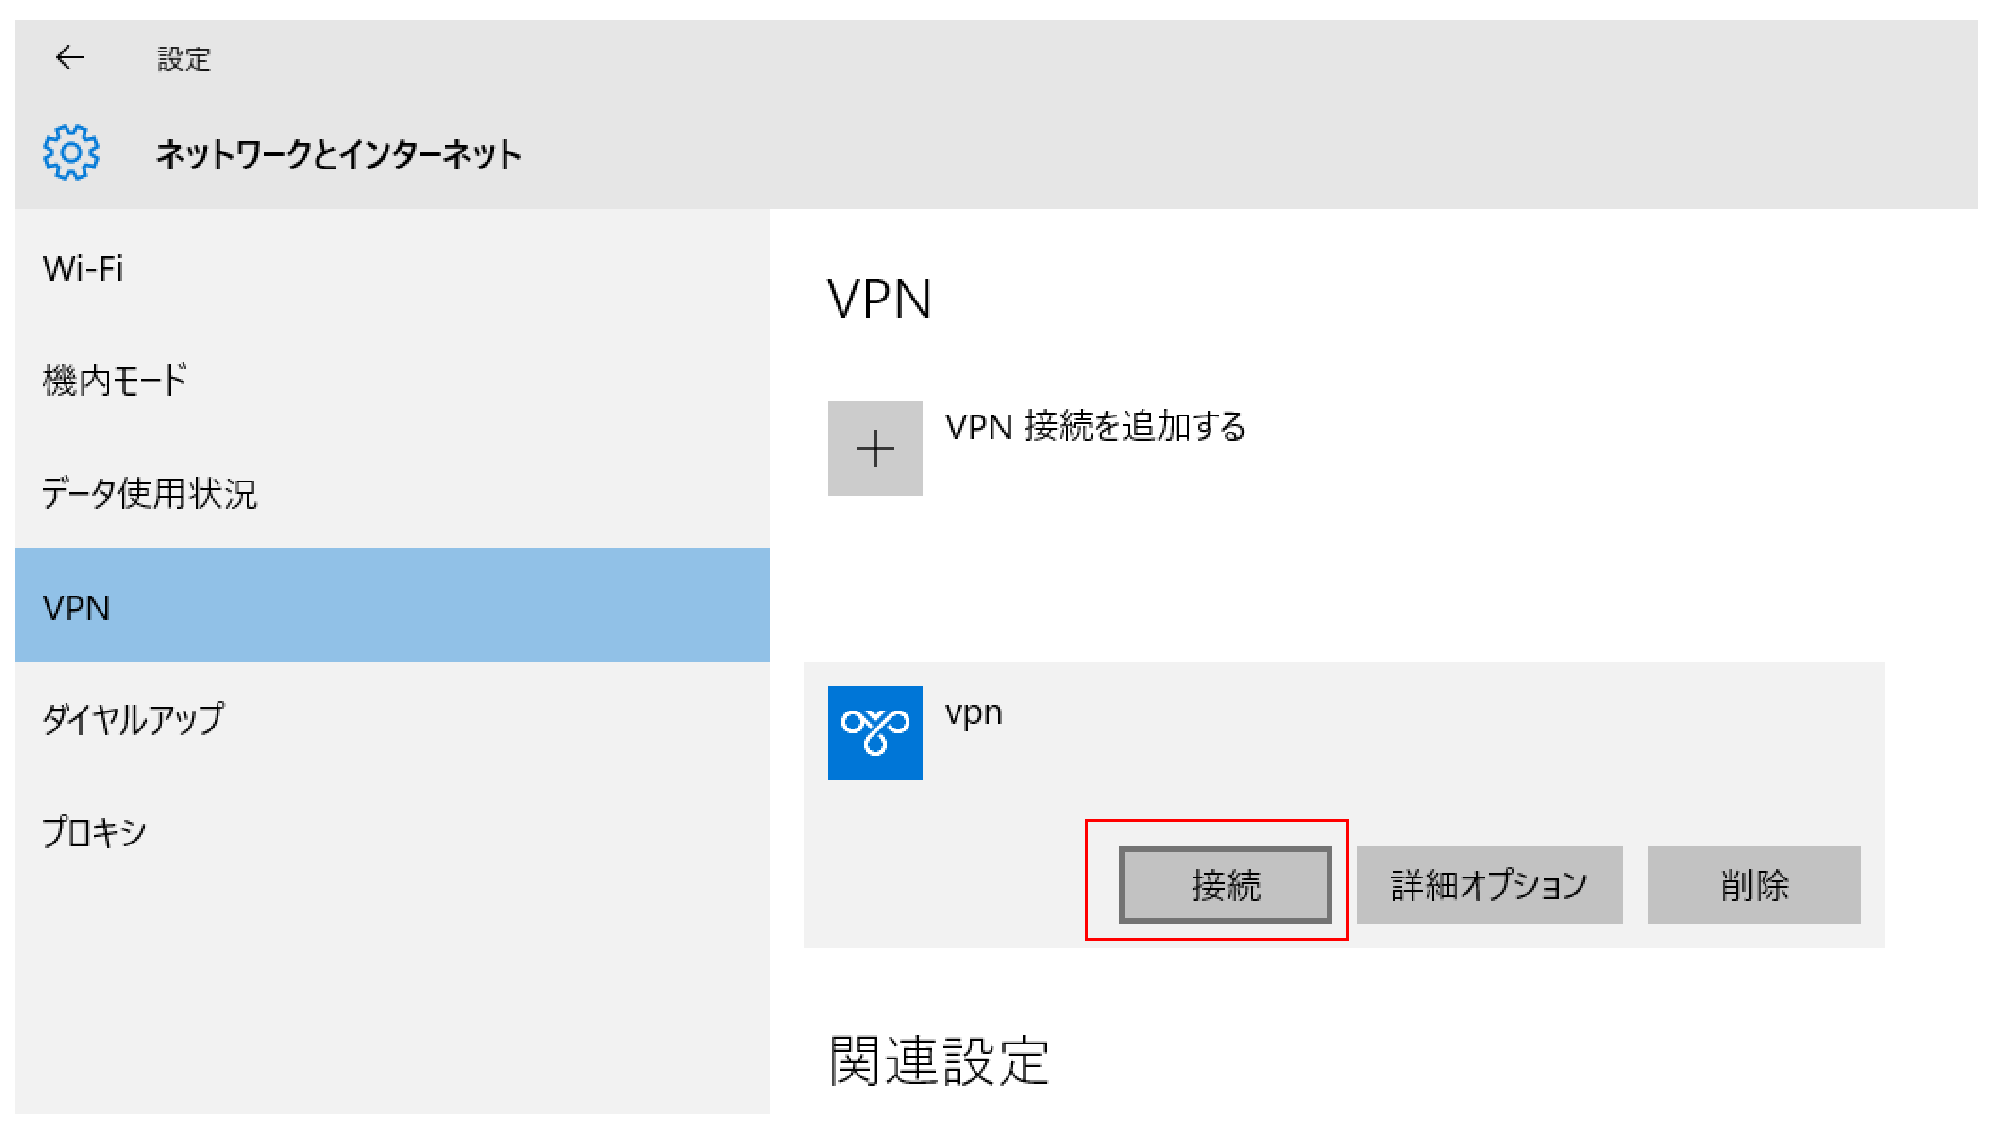
\includegraphics[width=15cm]{win-vpn8.pdf}
 \end{center}
 \caption{VPNの設定8}
 \label{winvpn8}
\end{figure}